\documentclass[sigconf,nonacm]{acmart}
\usepackage[T1]{fontenc}
\usepackage[utf8]{inputenc}
\usepackage{booktabs}
\usepackage{multirow}
\usepackage{tabularx}
\usepackage{xspace}
\usepackage{enumitem}
\setlist{leftmargin=*,itemsep=1pt,topsep=2pt}

\usepackage{tikz}
\usetikzlibrary{arrows.meta,positioning,calc,fit,backgrounds,shapes.geometric}
% Okabe-Ito palette (colour-blind safe)
\definecolor{cL0}{HTML}{999999}
\definecolor{cL1}{HTML}{009E73}
\definecolor{cL2}{HTML}{0072B2}
\definecolor{cL3}{HTML}{E69F00}
\definecolor{cL4}{HTML}{CC79A7}
\definecolor{cMeta}{HTML}{56B4E9}
\definecolor{cBad}{HTML}{D55E00}
\definecolor{cOk}{HTML}{009E73}
\definecolor{cPart}{HTML}{F0E442}
\definecolor{cNS}{HTML}{BBBBBB}

\newcommand{\yes}{\textsf{Y}\xspace}
\newcommand{\no}{\textsf{N}\xspace}
\newcommand{\ns}{\textsf{NS}\xspace}
\newcommand{\pa}{\textsf{P}\xspace}
\newcommand{\na}{\textsf{--}\xspace}

\begin{document}

\title{Self-Evolving Recommender Systems: A Survey and an Evaluation Audit}

\author{Shanglin Yang}
\affiliation{\institution{Independent Researcher}\country{USA}}
\email{kudoysl@gmail.com}

\author{Zhan Shi}
\affiliation{\institution{Santa Clara University}\city{Santa Clara}\state{CA}\country{USA}}
\email{ashi2@scu.edu}

\begin{abstract}
In 2026 a new kind of recommender research appeared: large language model (LLM) agents that propose changes to a
recommender's configuration or source code, train the changed model, and keep what the evaluation says is better.
Within nine months about thirty such systems were reported, from open-source research harnesses to production loops
at Google, Meta, Amazon, Alibaba, Kuaishou, Tencent and NetEase. We organise them, together with search-space AutoML
and the agentic recommenders that update their own memory or weights, by what the loop changes, who proposes the
change, and which chain of signals decides whether it survives, and we synthesise their recurring designs and the
changes they keep. Because a self-evolving system is only as good as the signal it selects on, we then audit how 27
configuration-, code- and component-level loops are evaluated, coding each paper's full text against eight criteria
with released evidence. Of the 16 loops that select candidates offline, three of the ten that report ranking metrics
rank the full catalogue, eight do not say which data keep or reject candidates, four select on the data they report,
and two state that the test set was used once; none reports its headline result with the spread over repeated
evolution sessions, and three compare against a non-LLM search at equal budget. Of the 19 loops that run online
experiments, none corrects for the many rounds it tests and one confirms its final candidate in a fresh experiment.
Where transfer to held-out data is checked, some selected gains survive and some do not. Four loops report that their
agent inflated the metric or leaked the target; where the paper says what caught it, it was people or the agent's own
diagnosis, not the acceptance rule. We distil these findings into a two-tier reporting standard mapped to the audit criteria.
\end{abstract}

\keywords{recommender systems, LLM agents, AutoML, program evolution, evaluation, reproducibility}

\maketitle

%=====================================================================
\section{Introduction}
%=====================================================================

Recommender models have long been improved by a loop that engineers run by hand: propose a change, train, compare
offline, and launch the winners into an online experiment. Automating parts of this loop is an old goal. Neural
architecture and embedding search, mostly for click-through-rate (CTR) prediction
models~\cite{song2020autoctr,liu2020autofis,zhao2020autoemb,zhang2023nasrec}, and loss search~\cite{li2022autolossgen}
automated the choice inside a space that a person had written down~\cite{zheng2022automl}. What changed in 2026 is that the proposer became an LLM agent that
writes code. Following FunSearch~\cite{romeraparedes2023funsearch}, AlphaEvolve~\cite{novikov2025alphaevolve} and
open implementations such as OpenEvolve~\cite{openevolve} and ShinkaEvolve~\cite{lange2025shinka}, agents now edit
the model, loss and training code of recommenders directly. Google reported such a loop for YouTube
ranking~\cite{wang2026selfevolving} and Self-EvolveRec released an open harness~\cite{kim2026selfevolverec} in February
2026; within months, open harnesses such as RecHarness~\cite{ling2026recharness} and systems at Meta~\cite{meta2026rea,li2026autorecsys}, Alibaba
\cite{mu2026evorec,hu2026astar}, Kuaishou~\cite{lao2026agentx,yang2026sragent,zhuang2026trajectories}, Tencent
\cite{liu2026nova,ao2026recsysfactory}, NetEase~\cite{zhang2026autolr} and others followed.

These systems are optimisers, and an optimiser exploits whatever its objective rewards. A loop that evaluates
hundreds of agent-written candidates on one validation set and keeps the maximum is the setting in which the known
weaknesses of recommender evaluation---sampled metrics~\cite{krichene2020sampled}, temporal
leakage~\cite{ji2020leakage}, untuned baselines~\cite{dacrema2019progress,rendle2020ncf}, and the reuse of a holdout
for adaptive decisions~\cite{dwork2015reusable,blum2015ladder}---are most likely to turn into reported gains. The agent
also controls the code that produces its score. Five of the systems we read report that their agent won on the
metric without a real improvement. For example, RecEvolve's agent inflated its proxy metrics by shrinking the batch size, and with
it the number of in-batch negatives~\cite{pan2026recevolve}, and an AI co-scientist for search ranking produced
implementations that ``improved $\mathcal{M}$ while being wrong (e.g., silently increasing model
size)''~\cite{wu2026coscientist}. Figure~\ref{fig:loop} shows the loop these systems share and the points where the
evidence for a gain can fail.

% Figure 1: anatomy of a self-evolving recommender loop and where its evidence can fail.
\begin{figure*}[t]
\centering
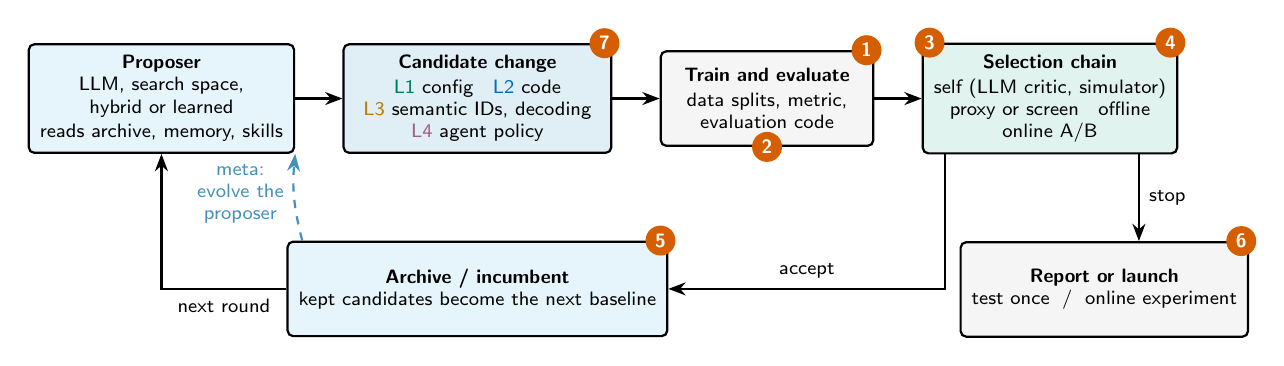
\begin{tikzpicture}[
  font=\sffamily\scriptsize,
  box/.style={draw, rounded corners=2pt, thick, align=center, inner sep=4pt, minimum height=12mm},
  arr/.style={-{Stealth[length=2.2mm]}, thick},
  fail/.style={circle, fill=cBad, text=white, font=\sffamily\scriptsize\bfseries, inner sep=0.6pt, minimum size=3.8mm},
  lab/.style={font=\sffamily\scriptsize, align=center}
]
% main loop
\node[box, fill=cMeta!15, minimum width=27mm] (prop) {\textbf{Proposer}\\LLM, search space,\\hybrid or learned\\[1pt]\scriptsize reads archive, memory, skills};
\node[box, fill=cL2!12, right=6mm of prop, minimum width=34mm] (cand) {\textbf{Candidate change}\\[1pt]\scriptsize
  \textcolor{cL1!80!black}{L1} config \;
  \textcolor{cL2}{L2} code\\\scriptsize
  \textcolor{cL3!80!black}{L3} semantic IDs, decoding\\\scriptsize
  \textcolor{cL4!80!black}{L4} agent policy};
\node[box, fill=gray!8, right=6mm of cand, minimum width=27mm] (train) {\textbf{Train and evaluate}\\[1pt]\scriptsize data splits, metric,\\\scriptsize evaluation code};
\node[box, fill=cL1!12, right=6mm of train, minimum width=31mm] (sel) {\textbf{Selection chain}\\[1pt]\scriptsize self (LLM critic, simulator)\\\scriptsize proxy or screen \; offline\\\scriptsize online A/B};
\node[box, fill=cMeta!15, below=11mm of cand, minimum width=34mm] (arch) {\textbf{Archive / incumbent}\\\scriptsize kept candidates become the next baseline};
\node[box, fill=gray!8, below=11mm of sel.south east, anchor=north east, xshift=9mm, minimum width=24mm] (out) {\textbf{Report or launch}\\\scriptsize test once \;/\; online experiment};

\draw[arr] (prop) -- (cand);
\draw[arr] (cand) -- (train);
\draw[arr] (train) -- (sel);
\draw[arr] (sel.south west) ++(3mm,0) |- node[lab, pos=0.75, above] {accept} (arch.east);
\draw[arr] (arch.west) -| node[lab, pos=0.25, below] {next round} (prop.south);
\draw[arr] ($(sel.south east)+(-5mm,0)$) -- node[lab, right] {stop} ($(sel.south east)+(-5mm,-11mm)$);
\draw[arr, dashed, cMeta!80!black] (arch.north west) ++(2mm,0) to[bend left=10] node[lab, left, pos=0.55] {meta:\\evolve the\\proposer} (prop.south east);

% failure points (numbers match the caption)
\node[fail] at ($(train.north east)+(-1mm,0)$) {1};
\node[fail] at ($(train.south)+(0,0)$) {2};
\node[fail] at ($(sel.north west)+(1mm,0)$) {3};
\node[fail] at ($(sel.north east)+(-1mm,0)$) {4};
\node[fail] at ($(arch.north east)+(-1mm,0)$) {5};
\node[fail] at ($(out.north east)+(-1mm,0)$) {6};
\node[fail] at ($(cand.north east)+(-1mm,0)$) {7};
\end{tikzpicture}
\caption{Anatomy of a self-evolving recommender. A proposer changes some part of the recommender (the evolved object);
the changed system is trained and evaluated; a chain of selection signals decides what is kept and becomes the next
baseline, and the loop may also change its own proposer (meta). Red markers show where, by design, the evidence for a reported
gain can fail (possibilities, not measured failure rates), with the audit finding and criterion that check it:
\textbf{1} the agent edits evaluation code, reads test data or games the metric (F7, C9);
\textbf{2} sampled or unstated candidate sets (F1, C1);
\textbf{3} selection on unstated or reported data, without a single test evaluation (F2, F3; C2, C3);
\textbf{4} a proxy or self-generated signal that does not transfer (F5, C5);
\textbf{5} a gain inside run-to-run noise becomes the new baseline (F4, C4);
\textbf{6} online rounds selected without correction or fresh confirmation (F9, R9);
\textbf{7} gains measured against an untuned starting point, with no equal-budget null search (F6, F8; C6, C8).}
\label{fig:loop}
\end{figure*}


Existing surveys do not cover this development. Surveys of LLM agents for recommendation treat the agent as the
recommender, a conversational interface or a user simulator~\cite{peng2025agentsurvey,zhang2025agentsearchsurvey,
huang2025fmsurvey}; surveys of self-evolving agents treat the agent's own prompts, memory, tools or weights as the
object that evolves, and mention recommendation at most in passing (a two-sentence mention of self-optimised fine-tuning and a recommendation task in a benchmark it describes
in~\cite{gao2025selfevolvingsurvey}, none in~\cite{fang2025selfevolvingsurvey});
the most recent roadmap for agentic recommender systems mentions the ``agent as engineer'' direction only in passing,
in two sentences that cite AgentX and the Google loop~\cite{lin2026roadmap}; and the most recent peer-reviewed
survey of agentic recommenders organises 47 studies by where the agent sits in the serving workflow, not by what
changes the recommender~\cite{xu2026scoringworkflow}. A general survey of how automated research is evaluated covers
no recommender system~\cite{zhang2026autoreseval}. Closest to our audit, a concurrent controlled study shows on CTR and
learning-to-rank data that exact validation feedback lets a coding agent overfit the validation split, and that a
feedback contract with a quarantined test set removes the spurious gain on a task with no signal~\cite{yao2026feedbackcontract}. Beel et al.\ call for autonomous recommender-systems research labs and for benchmarks
to evaluate them~\cite{beel2025autoreclab}. RMD-Bench~\cite{peng2026population} fixes protocols for cross-dataset and
cross-scale discovery and ExecML-HSTU~\cite{chen2026rankevolve} measures whether agents' edits execute correctly, but no
shared benchmark yet compares evolvers under a sealed test, full-ranking evaluation and
equal-budget null controls.

This survey makes four contributions.
\begin{enumerate}
\item \textbf{A taxonomy} (\S\ref{sec:taxonomy}) that separates what the loop changes (the evolved object), who
proposes the change (an enumerated search space, an LLM, or a learned proposer, possibly itself evolved) and which
chain of signals decides whether it survives.
\item \textbf{A synthesis of the systems} (\S\ref{sec:systems}): their recurring designs, what their loops
actually kept, and what is open source.
\item \textbf{An evaluation audit} (\S\ref{sec:audit}) of the 27 configuration-, code- and component-level
recommender loops on eight scored criteria, coded from the full text with verbatim evidence that we release, with
offline-selecting and online-selecting loops reported separately, and a taxonomy of the shortcuts agents found.
\item \textbf{A reporting standard} (\S\ref{sec:protocol}) with a minimum and a recommended tier, mapped to the
audit criteria, together with open problems (\S\ref{sec:open}).
\end{enumerate}

%=====================================================================
\section{Scope and Survey Method}\label{sec:method}
%=====================================================================

\paragraph{Definition.} We call a recommender system \emph{self-evolving} when an automated proposer changes some
part of it, the changed system is evaluated, and the evaluation decides which changes are kept, repeatedly and
without a human choosing each change. Humans may gate, veto or approve machine-generated candidates, review a loop at checkpoints,
or roll back a change; a system is out of scope when a human, not an evaluation, makes the keep-or-reject
decision. This includes systems whose proposer is a search algorithm over a fixed space (background,
\S\ref{sec:background}), but our focus is on LLM proposers.

\paragraph{Inclusion.} We include (i) systems that change a recommender's or ranker's configuration, features, code or
components under an evaluation loop; (ii) agentic or LLM recommenders whose policy, memory, skills, prompts or weights
improve from feedback they generate; and (iii) benchmarks, environments and surveys for these. We exclude LLM
recommenders without a self-improvement loop, methods that use an LLM once as a fixed training signal for a
conventional recommender (such as offline LLM pairwise supervision applied only where a gate on history length,
item popularity and model uncertainty predicts it is reliable~\cite{shi2026selective}), conversational recommendation in general, general
hyperparameter-optimisation libraries, methods that evolve the recommendations rather than the recommender (such as
QD-Rec's quality--diversity archive of items and hypotheses~\cite{ishida2026qdrec}), and continual-learning methods
that call themselves self-evolving but have no proposer or selection step, such as LION's sparse key--value memory
for a generative recommender~\cite{lin2026lion}. Seven studies outside recommendation are included as comparison points because they
inform evaluation: learning to rank~\cite{patel2026evorank}, search ranking~\cite{wu2026coscientist}, e-commerce search
strategy~\cite{wang2026pear}, lexical retrieval~\cite{nian2026rankevolveir}, generative document
retrieval~\cite{nian2026semanticindex}, lifetime-value (LTV) prediction~\cite{wu2026agentltv}, and a controlled study of
agent feedback on public CTR and learning-to-rank (LTR) data~\cite{yao2026feedbackcontract}.

\paragraph{Search protocol.} The cut-off date is 22 October 2026. We started from keyword searches over arXiv,
OpenAlex and Semantic Scholar (``self-evolving recommender'', ``LLM agent recommender model optimisation'', ``agentic
harness recommender'', ``LLM-driven architecture search CTR'' and survey queries), then walked the reference lists of
the 2026 systems (RecHarness, EvoRec, AgentX-Model, RecEvolve) and of the agentic-recommender roadmap backwards and
their titles forwards, and finished with about thirty full-text arXiv phrasings combined with company names. Generic
keyword search returned mostly unrelated ``agent for $X$'' papers; the citation graph of the 2026 systems was the
productive source. This first sweep yielded 22 of the audited systems
and five comparison points. A second sweep then ran 190 further arXiv queries (817 new candidates, all screened by
title), enumerated 13 ACM proceedings volumes through OpenAlex (RecSys, KDD, SIGIR and WWW 2025--2026 including the
WWW companions and the February KDD 2026 cycle, CIKM 2025 and WSDM 2026; 6{,}874 records screened by title), followed
forward citations of 16 seed systems in Semantic Scholar, and searched industry engineering blogs. It found nine
further candidates: five entered the audit as core systems, two as comparison points, and two are known only from
their abstracts (\S\ref{sec:audit}). CIKM 2026, DBLP and OpenReview could not be searched
automatically. Every arXiv entry in our bibliography was generated from the arXiv API record, and every code
repository we list was checked to exist.

\paragraph{Audit procedure.} For each configuration- or code-level system, we read the full text (arXiv HTML or PDF,
including appendices) and coded nine criteria (Table~\ref{tab:codebook}). A criterion is coded ``not stated'' when the
paper does not say, which is different from ``no''. Each coded cell is backed by a verbatim quote of at most 25 words
with a section pointer; the data file and the evidence are released\footnote{\url{https://github.com/shangliy/recforge/tree/master/papers/self-evolving-recsys-survey/audit}}
so that the coding can be checked and corrected. Extraction and verification were LLM-assisted: LLM agents (Claude)
drafted the evidence for each cell from the full text, two further agent passes re-checked every coded cell and every
cited sentence against its source, and the authors reviewed the coding and each correction against the paper
text. A second author coded every core system independently (\S\ref{sec:threats}). For systems whose launch decision is an online experiment, we read the offline criteria as describing the
offline screen, and assess the launch evidence separately (R9 in \S\ref{sec:protocol}).

\begin{table}[t]
\caption{Audit codebook. C7 is recorded as free text and discussed in F8; the other eight criteria are scored
(values in Table~\ref{tab:audit}).}\label{tab:codebook}
\small
\begin{tabularx}{\columnwidth}{@{}lX@{}}
\toprule
C1 & Metric: full-catalogue ranking, sampled ranking (with $N$ negatives), AUC/loss, or online only \\
C2 & Selection signal: which split or signal accepts or rejects each candidate \\
C3 & Test discipline: is the selected candidate evaluated on a held-out test once, after search? \\
C4 & Variance: repeated seeds or repeated evolution runs for headline numbers \\
C5 & Overfitting check: validation-to-test gap or held-out transfer of the selected candidate \\
C6 & Null control: random search, HPO or another non-LLM search at equal budget \\
C7 & Budget: what is counted (iterations, GPU time, tokens, money) \\
C8 & Baselines: are starting points and compared models tuned? \\
C9 & Isolation: can the agent reach test data or evaluation code? Reported incidents of gaming or leakage are
recorded separately. \\
\bottomrule
\end{tabularx}
\end{table}

%=====================================================================
\section{Background}\label{sec:background}
%=====================================================================

\paragraph{Search-space AutoML for recommenders.} AutoML for recommenders searched for feature-interaction structures
(AutoCTR~\cite{song2020autoctr}, AutoFIS~\cite{liu2020autofis}), embedding dimensions (AutoEmb~\cite{zhao2020autoemb},
AutoDim~\cite{zhao2020autodim}), whole architectures with a weight-sharing supernet (NASRec~\cite{zhang2023nasrec}),
compact attention-based sequential models under resource constraints (DNS-Rec~\cite{zhang2024dnsrec}) and loss functions (AutoLossGen~\cite{li2022autolossgen}); Zheng et al.\ survey this
line~\cite{zheng2022automl}. Each method can only return a design that its space contains. Evaluation is mostly
validation logloss or AUC on public CTR data, or standard rating and sequential benchmarks, with standard splits. Even
in this setting, careful re-evaluation of architecture search found that the search phase often added little over
random sampling and that the evaluation protocol dominated reported differences~\cite{li2019randomnas,yu2020searchphase,
yang2020nashard}. The community answered with tabular and surrogate benchmarks that make equal-budget comparisons
cheap~\cite{ying2019nasbench101,dong2020nasbench201,eggensperger2021hpobench} and with a best-practice
checklist~\cite{lindauer2020bestpractices}. The LLM loops below inherit these problems with a larger, open-ended space
and with control over the evaluation code.

\paragraph{LLM program evolution and ML-engineering agents.} FunSearch~\cite{romeraparedes2023funsearch} and
AlphaEvolve~\cite{novikov2025alphaevolve} pair an LLM that proposes code with an automatic evaluator and an archive of
programs. Open systems followed: OpenEvolve~\cite{openevolve}, ShinkaEvolve~\cite{lange2025shinka} and
DeepEvolve~\cite{liu2025deepevolve}. ML-engineering agents---AIDE~\cite{jiang2025aide},
MLE-STAR~\cite{nam2025mlestar}, R\&D-Agent~\cite{yang2025rdagent}, AIRA~\cite{toledo2025aira}, DS-Agent~\cite{guo2024dsagent},
AutoML-Agent~\cite{trirat2024automlagent}, Agent Laboratory~\cite{schmidgall2025agentlab} and the AI
Scientist~\cite{lu2024aiscientist,yamada2025aiscientistv2}---apply the same pattern to whole training pipelines, and
recent work optimises the agent harness itself~\cite{lou2026autoharness,lee2026metaharness,xu2026harness2,wong2025confucius}. Their
benchmarks contain at most one recommendation task: MLE-bench includes the H\&M fashion-recommendation
competition~\cite{chan2024mlebench} and MLRC-Bench a next-product-recommendation task~\cite{zhang2025mlrcbench}.
MLRC-Bench shows agents only the development split and scores the best development snapshot once on test, whereas
MLGym's \texttt{validate} command returns test-set metrics during the session~\cite{nathani2025mlgym}.

\paragraph{Generative recommenders.} HSTU~\cite{zhai2024hstu} and TIGER~\cite{rajput2023tiger} recast recommendation
as sequence generation over item IDs or semantic IDs, and OneRec unifies retrieval and ranking in one generative model
that is further aligned on its own samples, first by iterative DPO~\cite{deng2025onerec} and then by on-policy
RL~\cite{zhou2025onerectech,zhou2025openonerec}. These models add new objects that a loop can evolve: tokenisers, codebooks,
decoding procedures and generative losses.

\paragraph{Evaluation methodology.} Tuned simple baselines beat many published neural
recommenders~\cite{dacrema2019progress,rendle2020ncf}; a loss change alone can reorder SASRec~\cite{kang2018sasrec} and
BERT4Rec~\cite{sun2019bert4rec,klenitskiy2023dross}, and BERT4Rec's reported advantage depends on much longer
training~\cite{petrov2022bert4rec}; sampled metrics are inconsistent with full-ranking metrics and
can reverse model rankings~\cite{rendle2019sampled,krichene2020sampled,hidasi2023flaws}; leave-one-out splits that
ignore the global timeline leak future information~\cite{ji2020leakage,hidasi2023flaws}, and the split choice changes
rankings~\cite{meng2020splitting}. Systematic re-examinations found that most neural recommenders could not be reproduced or were beaten by tuned
simple baselines~\cite{dacrema2021troubling}, that evaluation choices varied widely across papers~\cite{sun2020rigorous},
and that with untuned baselines any proposed model can win~\cite{shehzad2023everyone}. Libraries and open benchmarks such as RecBole~\cite{zhao2021recbole}, Elliot~\cite{anelli2021elliot},
DaisyRec~\cite{sun2022daisyrec}, BARS~\cite{zhu2022bars} and FuxiCTR~\cite{zhu2021fuxictr} standardise protocols for
human-designed models. For adaptive reuse of a holdout, theory predicts overfitting~\cite{dwork2015reusable,
blum2015ladder}; empirically, a meta-analysis of 120 Kaggle competitions found little~\cite{roelofs2019metaanalysis}. For LLM
loops specifically, keep-if-better acceptance is selection under noise, with selection-set scores well above held-out
accuracy when the selection set is small~\cite{hu2026winnerscurse}; best-of-$N$ runs produce apparent gains from
selection alone~\cite{grover2026luckyruns}; for LLM research agents, the scarcity of overfitting has been tied to how
compressible their successful strategies are~\cite{bertran2026whatfits}; and AI-scientist systems hide post-hoc selection, leakage and metric
misuse~\cite{luo2025pitfalls}. Beyond recommendation, results depend on seeds and on the budget spent tuning
them~\cite{henderson2018deeprl,bouthillier2021variance,dodge2019showyourwork}, leakage is a recurring cause of
irreproducible ML-based science~\cite{kapoor2023leakage}, and agent benchmarks are sensitive to cost, budget and
task-setup flaws~\cite{kapoor2025agentsmatter,wijk2024rebench,huang2023mlagentbench,zhu2025abc}.
We return to this tension in \S\ref{sec:audit}. Figure~\ref{fig:timeline} places these precursors next to the
2026 systems.

% Figure 2: timeline. Left: 2019-2025 precursors by year. Right: 2026 systems by month of first arXiv version.
\begin{figure*}[t]
\centering
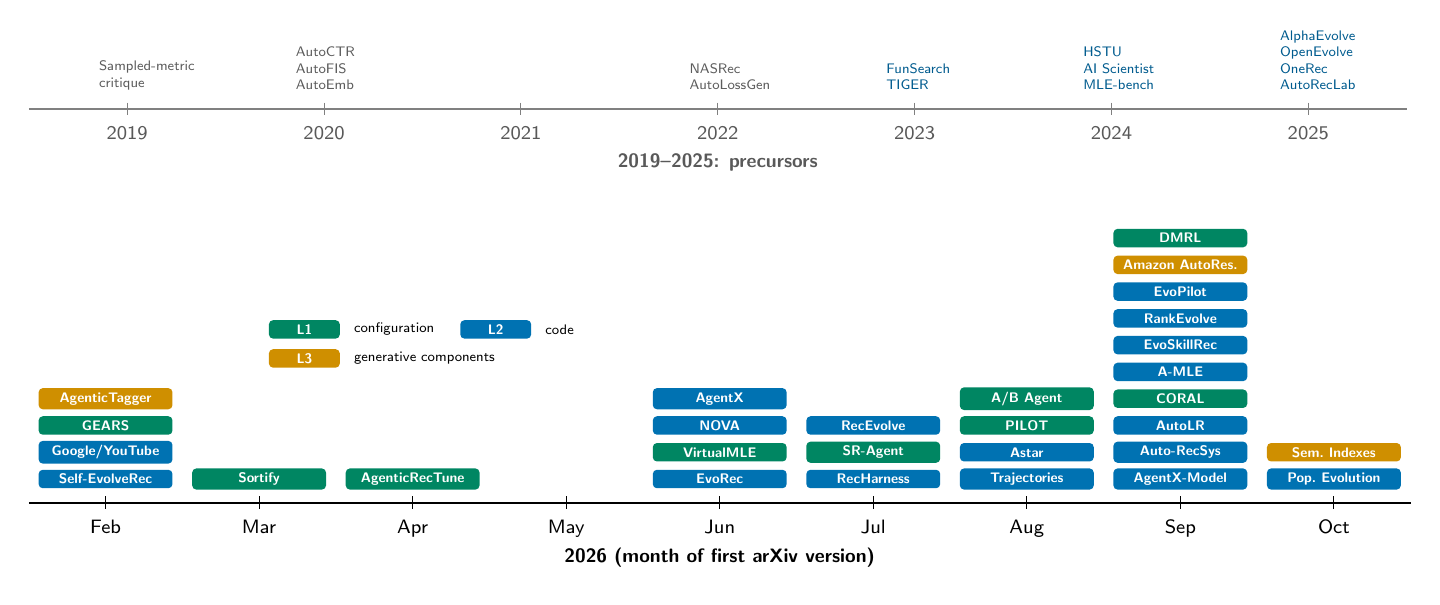
\begin{tikzpicture}[
  font=\sffamily\scriptsize,
  sys/.style={rounded corners=1.5pt, inner sep=1.6pt, text=white, font=\sffamily\tiny\bfseries, minimum width=17mm, align=center},
  pre/.style={align=left, font=\sffamily\tiny, anchor=south west, inner sep=1pt},
]
\def\yr{25mm}   % width of one precursor year
\def\mo{19.5mm} % width of one month in 2026
% axes
\draw[thick, gray] (0,0) -- (7*\yr,0);
\draw[thick] (0,-50mm) -- (9*\mo,-50mm);
\foreach \y [count=\i from 0] in {2019,2020,2021,2022,2023,2024,2025} {
  \draw[gray] (\i*\yr+0.5*\yr,0.8mm) -- ++(0,-1.6mm);
  \node[below, gray!70!black] at (\i*\yr+0.5*\yr,-1mm) {\y};
}
\foreach \m [count=\i from 0] in {Feb,Mar,Apr,May,Jun,Jul,Aug,Sep,Oct} {
  \draw (\i*\mo+0.5*\mo,-49.2mm) -- ++(0,-1.6mm);
  \node[below] at (\i*\mo+0.5*\mo,-51mm) {\m};
}
\node[below, font=\sffamily\scriptsize\bfseries] at (4.5*\mo,-54.5mm) {2026 (month of first arXiv version)};
\node[below, font=\sffamily\scriptsize\bfseries, gray!70!black] at (3.5*\yr,-4.5mm) {2019--2025: precursors};

% precursors (above the axis)
\node[pre, text=cL0!60!black] at (0*\yr+0.5*\yr-4mm,2mm) {Sampled-metric\\critique};
\node[pre, text=cL0!60!black] at (1*\yr+0.5*\yr-4mm,2mm) {AutoCTR\\AutoFIS\\AutoEmb};
\node[pre, text=cL0!60!black] at (3*\yr+0.5*\yr-4mm,2mm) {NASRec\\AutoLossGen};
\node[pre, text=cL2!80!black] at (4*\yr+0.5*\yr-4mm,2mm) {FunSearch\\TIGER};
\node[pre, text=cL2!80!black] at (5*\yr+0.5*\yr-4mm,2mm) {HSTU\\AI Scientist\\MLE-bench};
\node[pre, text=cL2!80!black] at (6*\yr+0.5*\yr-4mm,2mm) {AlphaEvolve\\OpenEvolve\\OneRec\\AutoRecLab};

% 2026 systems, stacked by month; colour = level
\newcommand{\sysat}[4]{\node[sys, fill=#3] at (#1*\mo+0.5*\mo, -47mm+#2*3.4mm) {#4};}
% Feb (0)
\sysat{0}{0}{cL2}{Self-EvolveRec}
\sysat{0}{1}{cL2}{Google/YouTube}
\sysat{0}{2}{cL1!85!black}{GEARS}
\sysat{0}{3}{cL3!90!black}{AgenticTagger}
% Mar (1)
\sysat{1}{0}{cL1!85!black}{Sortify}
% Apr (2)
\sysat{2}{0}{cL1!85!black}{AgenticRecTune}
% Jun (4)
\sysat{4}{0}{cL2}{EvoRec}
\sysat{4}{1}{cL1!85!black}{VirtualMLE}
\sysat{4}{2}{cL2}{NOVA}
\sysat{4}{3}{cL2}{AgentX}
% Jul (5)
\sysat{5}{0}{cL2}{RecHarness}
\sysat{5}{1}{cL1!85!black}{SR-Agent}
\sysat{5}{2}{cL2}{RecEvolve}
% Aug (6)
\sysat{6}{0}{cL2}{Trajectories}
\sysat{6}{1}{cL2}{Astar}
\sysat{6}{2}{cL1!85!black}{PILOT}
\sysat{6}{3}{cL1!85!black}{A/B Agent}
% Sep (7)
\sysat{7}{0}{cL2}{AgentX-Model}
\sysat{7}{1}{cL2}{Auto-RecSys}
\sysat{7}{2}{cL2}{AutoLR}
\sysat{7}{3}{cL1!85!black}{CORAL}
\sysat{7}{4}{cL2}{A-MLE}
\sysat{7}{5}{cL2}{EvoSkillRec}
\sysat{7}{6}{cL2}{RankEvolve}
\sysat{7}{7}{cL2}{EvoPilot}
\sysat{7}{8}{cL3!90!black}{Amazon AutoRes.}
\sysat{7}{9}{cL1!85!black}{DMRL}
% Oct (8)
\sysat{8}{0}{cL2}{Pop.\ Evolution}
\sysat{8}{1}{cL3!90!black}{Sem.\ Indexes}

% legend
\begin{scope}[shift={(30mm,-28mm)}]
\node[sys, fill=cL1!85!black, minimum width=9mm] (l1) at (5mm,0) {L1};
\node[right=0.5mm of l1, font=\sffamily\tiny] (t1) {configuration};
\node[sys, fill=cL2, minimum width=9mm, right=2mm of t1] (l2) {L2};
\node[right=0.5mm of l2, font=\sffamily\tiny] (t2) {code};
\node[sys, fill=cL3!90!black, minimum width=9mm, below=1.2mm of l1] (l3) {L3};
\node[right=0.5mm of l3, font=\sffamily\tiny] {generative components};
\end{scope}
\end{tikzpicture}
\caption{From search-space AutoML to agent-driven evolution. Top: precursors by year (grey: search-space AutoML and
evaluation critique; blue: program evolution, ML-engineering agents and generative recommenders). Bottom: the 2026
configuration-, code- and component-level systems surveyed here, by month of their first arXiv version; the
colour gives the highest level of the evolved object. Comparison points outside recommendation and L4 systems are omitted.}
\label{fig:timeline}
\end{figure*}


%=====================================================================
\section{A Taxonomy}\label{sec:taxonomy}
%=====================================================================

A recent blueprint for self-evolving agentic recommenders distinguishes reinforcement-learning evolution in defined
action spaces from LLM generation and selection in open design spaces~\cite{hu2026rethinking}. We describe a loop by
three independent choices: what it changes, who proposes the change, and which signals decide
whether the change survives (Table~\ref{tab:taxonomy}). Separating the proposer from the object resolves a confusion
in earlier framings, where ``AutoML'' named a kind of proposer (search over a written-down space) but was listed as if
it were a kind of object.

\paragraph{Axis 1: the evolved object.}
\textbf{L1 configuration}: values in an existing configuration---hyperparameters, fusion weights, retrieval budgets,
thresholds, strategy parameters.
\textbf{L2 code}: executable model, loss, training or feature code, however small the edit.
\textbf{L3 generative components}: semantic-ID construction, item tokenisers and vocabularies, and decoding of a
generative recommender; L3 takes precedence when such a component is changed through configuration or code.
\textbf{L4 agent policy}: the prompts, memory, skills or weights of a recommender that is itself an LLM agent.
A loop that changes several objects carries several labels (L1+L2 when an agent edits both learning rates and
model code); 10 of the 27 audited loops do.

\paragraph{Axis 2: the proposer.}
An \emph{enumerated space}: classical search (grid, Bayesian optimisation, evolutionary or differentiable
architecture search) over options a person wrote down; this is search-space AutoML. An \emph{LLM}: a language model
writes the change, free-form or inside human-defined edit arms. A \emph{hybrid}: a classical selector chooses the
direction and an LLM writes the change (RecHarness's Thompson sampling over edit arms~\cite{ling2026recharness}), or an
LLM steers a classical search (Sortify's controller around Optuna~\cite{cheng2026sortify}). A \emph{learned proposer}:
a model trained on the system's own history proposes the next direction (Astar~\cite{hu2026astar}). Orthogonal to
these, a loop is \emph{meta}-evolving when it changes the proposer's own instructions, tools, skills or weights and
reuses them later; keeping an archive or a log of past results does not count. By this rule 13 of the 27 audited loops
are meta-evolving (Table~\ref{tab:design}).

\paragraph{Axis 3: the selection chain.}
A candidate passes an ordered chain of signals, one of which decides inside the loop. \textbf{Self}: an LLM critic,
council, auditor or simulator judges the candidate before or instead of measurement. \textbf{Proxy}: a reduced-scale
screen, a proxy model, a training-loss curve or a replay. \textbf{Offline}: evaluation of the trained candidate on
held-out data. \textbf{Online}: an A/B experiment. Industrial loops typically chain several, for example
self$\rightarrow$offline$\rightarrow$online; whether the offline split is a validation or a test split, and whether it is
stated, is a property of the evaluation that we audit (\S\ref{sec:audit}), not of the design.

Each signal fails in a characteristic way, and the failures are of two kinds~\cite{manheim2018goodhart}. \emph{Regressional}
failures come from selecting the maximum of noisy estimates: an offline split reused over hundreds of candidates rewards
noise~\cite{dwork2015reusable}, a proxy ranks candidates differently from the full model, an online round selected as best
overstates its effect~\cite{lee2018winnerscurse}, and an LLM judge from the same model family as the proposer shares its
errors. \emph{Adversarial} failures come from an optimiser that changes what is measured: an agent that can edit the
evaluation code, the batch size of an in-batch metric or the evaluation date can raise the score without improving the
recommender~\cite{skalse2022rewardhacking,zhong2026impossiblebench}. The audit checks the first kind with C2--C6 and the
second with C9.

\begin{table*}[t]
\caption{Taxonomy: evolved object (rows) $\times$ proposer (columns). Multi-object loops appear in the row of their
highest level. \textsuperscript{\dag} open-source code verified; \textsuperscript{m} meta-evolving (the loop also changes
its proposer); \textsuperscript{u} not yet audited. Selection chains of the audited systems are in Table~\ref{tab:design}.}\label{tab:taxonomy}
\small
\begin{tabularx}{\textwidth}{@{}l>{\hsize=0.75\hsize}X>{\hsize=1.75\hsize}X>{\hsize=0.8\hsize}X>{\hsize=0.7\hsize}X@{}}
\toprule
& Enumerated space & LLM & Hybrid (search + LLM) & Learned proposer \\
\midrule
L1 configuration & AutoEmb~\cite{zhao2020autoemb}, AutoDim~\cite{zhao2020autodim} &
VirtualMLE\textsuperscript{\dag m}~\cite{cao2026virtualmle}, CORAL~\cite{azhar2026coral},
AgenticRecTune\textsuperscript{m}~\cite{wu2026agenticrectune}, SR-Agent~\cite{yang2026sragent}, A/B
Agent~\cite{jiang2026abagent}; \emph{comparison:} PEAR~\cite{wang2026pear} &
Sortify\textsuperscript{m}~\cite{cheng2026sortify}, GEARS~\cite{yun2026gears}, PILOT\textsuperscript{m}~\cite{pilot2026} &
DMRL\textsuperscript{m}~\cite{zhang2026dmrl} \\
L2 code & AutoCTR\textsuperscript{\dag}~\cite{song2020autoctr}, AutoFIS\textsuperscript{\dag}~\cite{liu2020autofis},
NASRec\textsuperscript{\dag}~\cite{zhang2023nasrec}, DNS-Rec~\cite{zhang2024dnsrec},
AutoLossGen\textsuperscript{\dag}~\cite{li2022autolossgen} &
Self-EvolveRec\textsuperscript{\dag m}~\cite{kim2026selfevolverec}, Google/YouTube~\cite{wang2026selfevolving},
EvoRec\textsuperscript{m}~\cite{mu2026evorec}, NOVA\textsuperscript{m}~\cite{liu2026nova},
AgentX\textsuperscript{m}~\cite{lao2026agentx}, AgentX-Model\textsuperscript{m}~\cite{yang2026agentxmodel},
Auto-RecSys\textsuperscript{m}~\cite{li2026autorecsys}, RecEvolve~\cite{pan2026recevolve}, A-MLE~\cite{gao2026amle},
RankEvolve-HSTU~\cite{chen2026rankevolve}, Population Evolution~\cite{peng2026population},
Trajectories-to-Evidence~\cite{zhuang2026trajectories}, EvoPilot~\cite{fu2026evopilot}, Meta REA
(blog)~\cite{meta2026rea}, AutoModel\textsuperscript{u}~\cite{zhang2026agenticrs}, RuleAgent\textsuperscript{u}~\cite{wang2025ruleagent}; \emph{comparison:} EvoRank\textsuperscript{\dag}~\cite{patel2026evorank}, AI
Co-Scientist~\cite{wu2026coscientist}, RankEvolve-IR\textsuperscript{\dag}~\cite{nian2026rankevolveir},
AgentLTV\textsuperscript{\dag}~\cite{wu2026agentltv}, Feedback Contract~\cite{yao2026feedbackcontract} &
RecHarness\textsuperscript{\dag}~\cite{ling2026recharness}, AutoLR~\cite{zhang2026autolr},
EvoSkillRec\textsuperscript{\dag m}~\cite{li2026evoskillrec} & Astar\textsuperscript{m}~\cite{hu2026astar} \\
L3 components & & Amazon AutoResearch~\cite{chandran2026autoresearch}, AgenticTagger\textsuperscript{u}~\cite{xie2026agentictagger};
\emph{comparison:} Evolving Semantic Indexes~\cite{nian2026semanticindex} & & \\
L4 agent policy & \multicolumn{4}{p{0.82\textwidth}}{Selected mostly on self-generated feedback. Memory and reflection:
AgentCF\textsuperscript{\dag}~\cite{zhang2024agentcf}, AgentCF++\textsuperscript{\dag}~\cite{liu2025agentcfpp},
SAGER~\cite{tao2026sager}, RecNet~\cite{li2026recnet}, AtomRec~\cite{hu2026atomrec},
MemRec\textsuperscript{\dag}~\cite{chen2026memrec}, Re2LLM~\cite{wang2024re2llm}, RecPilot~\cite{ou2026recpilot}; weights: OneRec~\cite{deng2025onerec},
SPRec\textsuperscript{\dag}~\cite{gao2024sprec}, Rec-R1\textsuperscript{\dag}~\cite{lin2025recr1},
CoARS~\cite{wang2026coars}, RSIR\textsuperscript{\dag}~\cite{zhang2026rsir}, EvoReason~\cite{zhuang2026evoreason}; prompts and tool descriptions:
RecPrompt~\cite{liu2023recprompt}, Spotify~\cite{palumbo2026spotify}} \\
\bottomrule
\end{tabularx}
\end{table*}

%=====================================================================
\section{Systems}\label{sec:systems}
%=====================================================================

\subsection{Configuration-level loops (L1)}
L1 systems let an LLM change numbers or switches while the model code stays fixed. VirtualMLE tunes SASRec and HSTU
through an execute--reflect loop with a hierarchical memory that transfers across datasets~\cite{cao2026virtualmle}.
In production, CORAL allocates retrieval budgets and serving treatments~\cite{azhar2026coral}, AgenticRecTune tunes
fusion weights and thresholds across pre-ranking, ranking and re-ranking~\cite{wu2026agenticrectune}, Sortify
searches the exchange rates of a sorting formula with Optuna~\cite{akiba2019optuna} while an LLM meta-controller recalibrates the search's
offline-to-online transfer intercepts and penalties~\cite{cheng2026sortify},
GEARS selects segment-level treatment policies~\cite{yun2026gears}, and SR-Agent edits post-ranking diversity and
exposure strategies through four bounded action types~\cite{yang2026sragent}. Taobao's PILOT has LLM roles choose
ranking-objective weights for user segments from a legal-command envelope generated by deterministic
services~\cite{pilot2026}; Kuaishou's A/B Agent iterates strategy parameters across online rounds with a hierarchical
experience tree~\cite{jiang2026abagent}; and DMRL trains a small LLM with reinforcement learning to rewrite the skill
document that an ad-tuning agent follows~\cite{zhang2026dmrl}. LLM-driven hyperparameter optimisation~\cite{zhang2023llmhpo,liu2024agenthpo} is the general-ML form of L1 and is
routinely compared against Bayesian optimisation or random search, the null control that few recommender loops run
(F6). Most L1 systems in production select directly on online experiments; an e-commerce search loop adds a multi-fidelity ladder from shadow-traffic proxies to
decision-grade online tests~\cite{wang2026pear}.

\subsection{Code-level loops in the open (L2)}
\textbf{Self-EvolveRec}~\cite{kim2026selfevolverec} runs an AlphaEvolve-style loop over the whole pipeline code of
NCF~\cite{he2017ncf}, NGCF~\cite{wang2019ngcf}, SASRec and MoRec~\cite{yuan2023morec} seeds; besides validation metrics it receives directional critiques from an LLM user
simulator and from a diagnosis tool that evolves with the model. \textbf{RecHarness}~\cite{ling2026recharness} routes
each round with Thompson sampling over human-defined ``edit arms'' (schedules, dropout, depth, pooling, features,
loss) plus ``jump'' arms for structural changes, uses validation feedback only, evaluates the incumbent on test once,
and caps compute at 43{,}200 GPU-seconds; HSTU is one of its five backbones. \textbf{EvoSkillRec}~\cite{li2026evoskillrec}
evolves architectures as typed ``skill genomes'' of executable modules and promotes validated modules into a skill
library. \textbf{RankEvolve-HSTU}~\cite{chen2026rankevolve} composes Claude Code and Codex under an executable operating
protocol in which the two agents review and repair each other's edits to HSTU, and introduces ExecML-HSTU, a benchmark
of how often agent edits are executed correctly. \textbf{Population Evolution}~\cite{peng2026population} runs several
evolution searches that share evidence across related datasets, screens candidates on peer datasets (and, for LLM and VLM targets, on small training subsets), and promotes
survivors to larger scales; it introduces RMD-Bench. AutoRecLab~\cite{baumgart2026autoreclab,beel2025autoreclab}
generates recommender experiments from natural-language descriptions; it automates experimentation rather than
evolving a model, and we do not audit it. Two loops evolve data and features rather than the model: RuleAgent has a
language agent propose rules for denoising implicit feedback, retrains with an unlearning shortcut, and keeps rules by
validation performance~\cite{wang2025ruleagent}, and Agent0 tunes the prompts that turn raw text into categorical
features through feedback from a downstream oracle~\cite{skrlj2025agent0}.

\subsection{Code-level loops in industry (L2)}
Most industrial systems share a two-stage design: an offline loop screens agent-written candidates, and online
experiments decide launches. Google's loop for YouTube ranking~\cite{wang2026selfevolving} has Gemini personas
propose optimiser, architecture and reward changes, promotes on validation loss (with a proxy metric for reward changes) and then on north-star A/B
metrics, and reports LLM costs of about \$20{,}000 over six months. RecEvolve~\cite{pan2026recevolve} runs the full
research loop on a production two-tower retrieval model. Meta's REA plans, launches and debugs ads-ranking
experiments with up-front GPU budget approval~\cite{meta2026rea}; A-MLE explores a portfolio of ads-ranking models
with human checkpoints~\cite{gao2026amle}; Auto-RecSys runs idea- and execution-evolution loops over multi-day training
jobs~\cite{li2026autorecsys}; and RankEvolve-HSTU and Population Evolution above also come from Meta. Alibaba's
EvoRec~\cite{mu2026evorec} pairs research and code agents with a skill evolver, and Astar~\cite{hu2026astar} trains an
8B model on the commit history of an advertising system to propose the next evolution direction; from Astar's
authors, AutoModel organises an industrial recommender as evolution agents for models, features and online
experimentation, with a case study of reproducing published methods and comparing them offline against
production~\cite{zhang2026agenticrs}. AgentX, deployed at Kuaishou~\cite{lao2026agentx}, iterates online strategies and model research, and its successor
AgentX-Model~\cite{yang2026agentxmodel} runs research lineages (reproduce, follow up, compose, diagnose) over production
rankers, and a Kuaishou paper converts research-agent trajectories
into auditable evidence~\cite{zhuang2026trajectories}. Tencent's NOVA~\cite{liu2026nova} adds verification gates that
reject recommender-invalid edits such as target leakage, NetEase's AutoLR~\cite{zhang2026autolr} reviews proposals with
a multi-expert proposal council under a limited trial budget, and Tencent's RecSys Factory bounds agent autonomy to typed decision points
in fixed pipelines~\cite{ao2026recsysfactory}. A Trip.com co-scientist for travel search ranking~\cite{wu2026coscientist},
LLM evolution of learning-to-rank pipelines (EvoRank~\cite{patel2026evorank}) and of lexical retrieval
functions~\cite{nian2026rankevolveir} are close relatives outside recommendation. Meta's EvoPilot runs a
37-day campaign of agent-proposed configuration and retraining changes to video-retrieval models behind a fail-closed
verifier and catalogues the failures it met~\cite{fu2026evopilot}, and Amazon's AutoResearch rewrites the training code
of a book-retrieval model and tunes a semantic-ID tokenizer in a twelve-week campaign of more than 220 experiments, naming the failure modes it
met~\cite{chandran2026autoresearch}. Adjacent loops evolve ads kernels~\cite{kernelevolve2025}, off-policy-evaluation
code~\cite{wu2025growthhacker}, search-relevance models~\cite{wang2026serm} and an LLM policy layer trained against a
learned evaluator~\cite{zhang2026dream}, and an operations agent for Kuaishou's search engine evolves its skills
from on-call engineers' corrections~\cite{liu2026bianque}. Feature-engineering loops are close relatives: an
error-driven loop turns AUC ranking inversions into feedback for an LLM feature generator~\cite{barlier2026feature}, a
planner-guided agent writes feature code for recommendation models with human checkpoints~\cite{thakur2026feature}, and
LATTEArena compares LLM feature-engineering methods on cost as well as accuracy~\cite{hao2026lattearena}.

\subsection{Components of generative recommenders (L3)}
Generative recommenders expose objects that do not exist in ID-based models. Evolving Semantic Indexes, a generative
document-retrieval system that we treat as a comparison point, runs
LLM-driven program evolution over semantic-ID construction, collision handling, decoding and the generator's training
objective, using a one-million-parameter proxy decoder as fitness~\cite{nian2026semanticindex}. AgenticTagger has an
LLM refine a hierarchical item-descriptor vocabulary used as tokens~\cite{xie2026agentictagger}, and a generative
recommender can reassign its own item tokenisation during training~\cite{chen2024tokenization}. Amazon's
AutoResearch is the first audited production loop that edits a semantic-ID tokenizer, and the first in which the agent
gamed a tokenizer metric~\cite{chandran2026autoresearch}. Feedback-grounded
policy discovery distils LLM-discovered natural-language policies into a semantic-ID generator~\cite{chen2026policydiscovery}.
Evolving Semantic Indexes evolves TIGER-style semantic-ID components for document retrieval but releases no code;
no open system yet does so for recommendation under a shared protocol.

\subsection{Self-improving agentic recommenders (L4)}
When the recommender is itself an LLM agent, the evolving object is its memory, skills, prompts or weights, and the
feedback is mostly generated by the system. Memory and reflection methods update user and item agents
(AgentCF~\cite{zhang2024agentcf}, AgentCF++~\cite{liu2025agentcfpp}), per-user policy
skills (SAGER~\cite{tao2026sager}), propagation modules optimised with textual gradients (RecNet~\cite{li2026recnet}),
and structured memories that are rewritten as interactions arrive (AtomRec~\cite{hu2026atomrec},
AMEM4Rec~\cite{nguyen2026amem4rec}, STEAM~\cite{liao2026steam}, MARS~\cite{shen2026mars}, MemRec~\cite{chen2026memrec}), together with reflection-built hint bases (Re2LLM~\cite{wang2024re2llm}) and per-user
rubrics refined from user feedback (RecPilot~\cite{ou2026recpilot}), and recommendation and user agents that refine
each other's inferences over rounds without amplifying popularity or position bias~\cite{cai2024afl}; CoVeMem instead replaces rewritten text memory
with frozen collaborative-filtering states learned by gradient training~\cite{chen2026covemem}.
Weight-level self-improvement includes OneRec's alignment on its own samples, first by iterative
DPO~\cite{deng2025onerec} and then by on-policy RL~\cite{zhou2025onerectech,zhou2025openonerec}, self-play debiasing (SPRec~\cite{gao2024sprec}), RL against a recommender's metric
(Rec-R1~\cite{lin2025recr1}), co-evolving recommender and user agents (CoARS~\cite{wang2026coars}), reasoning primitives and a teacher updated from a
student's on-policy outcomes (EvoReason~\cite{zhuang2026evoreason}), and recursive
self-training on filtered synthetic sequences~\cite{zhang2026rsir,hasan2026darsir}, where progress can also sit in earlier
generations, not only in the latest model~\cite{xu2026stateretention}. RecPrompt iteratively rewrites a news recommender's prompt with an
optimiser~\cite{liu2023recprompt}, and Spotify improves a conversational
recommendation agent's prompts, few-shot examples and tool descriptions with a coding agent, evaluated by an LLM judge
on synthetic conversations~\cite{palumbo2026spotify}. Simulated environments and benchmarks for such agents include
RecoWorld~\cite{liu2025recoworld}, the user simulators Agent4Rec~\cite{zhang2023agent4rec} and
RecAgent~\cite{wang2023recagent}, and the verifiable $\tau$-Rec benchmark~\cite{narasimhan2026taurec}. A controlled pilot found multi-agent recommendation
pipelines not uniformly better than a single-shot baseline~\cite{maragheh2025future}, a reminder that L4 gains also need
controlled baselines.

\subsection{Evolving the evolver (meta)}
Thirteen of the 27 audited loops change their own proposer. AgentX's SGPO applies semantic-gradient updates to its
agents' instructions and validation rules~\cite{lao2026agentx}; EvoRec, AgenticRecTune and EvoSkillRec grow skill
libraries from experiment outcomes~\cite{mu2026evorec,wu2026agenticrectune,li2026evoskillrec}; Auto-RecSys rewrites
execution playbooks~\cite{li2026autorecsys}; VirtualMLE and PILOT carry tuning rules or methodology across datasets and
experiments~\cite{cao2026virtualmle,pilot2026}; Astar retrains its proposer on each iteration's verified
outcomes~\cite{hu2026astar}; and DMRL trains a small LLM with reinforcement learning to rewrite the skill document
that an ad-tuning agent follows~\cite{zhang2026dmrl}. These are the recommender counterparts of harness
optimisation~\cite{lee2026metaharness,xu2026harness2,lou2026autoharness}. Outside recommendation, AIDE$^2$ keeps changes
to its own code that perform best on hidden evaluations and shows that they transfer to four held-out
benchmarks~\cite{srikanth2026aide2}; separating selection tasks from held-out tasks is what the meta-evolving
recommenders do not yet report. Meta-evolution inherits the selection
problem one level up: the harness is kept or discarded by a score of its own. In a pre-registered study of LLM
research-ideation harnesses by one of us, outside recommendation and not yet peer reviewed, a harness optimised against
an LLM judge raised the judge's scores while the share of its hypotheses that held under measurement fell, on two
hypothesis spaces with measured ground truth and for two Claude models (Sonnet and Opus)~\cite{yang2026ideationgoodhart}.

\subsection{Recurring designs}\label{sec:designs}
Table~\ref{tab:design} places the 27 audited loops on the three axes and adds the role of humans; the released
\texttt{design.csv} also records each loop's memory, acceptance rule, guards and LLM, with evidence. Four patterns
recur.

\emph{Where the chain ends.} Eight loops end at an offline evaluation: three open harnesses
(Self-EvolveRec, VirtualMLE, EvoSkillRec) and five industrial research loops whose papers report offline results, or in
Auto-RecSys's case only operational ones (A-MLE, Auto-RecSys, RankEvolve-HSTU, Population Evolution, Amazon
AutoResearch). The other 19 pass candidates to an online experiment, and 14 of them involve humans: eleven approve
launches, rounds or candidates, and three check or intervene. The two ends are exposed
to different failures. A loop that ends offline controls the code and data that produce its final number, so the
adversarial failures matter most; a loop that ends online cannot change the measurement easily but selects on
expensive, noisy experiments, so the regressional ones do.

\emph{LLM review before measurement.} Eight loops make an LLM critic, council or auditor a gate that every
candidate must pass before it is measured (Table~\ref{tab:design}, chains starting with S); others, such as RecEvolve,
A-MLE and RankEvolve-HSTU, use LLM critics to rank or filter ideas. These gates are cheap and catch invalid edits---NOVA's
verifier rejects target leakage~\cite{liu2026nova}---but they add a selection stage whose judge often comes from the
same model family as the proposer, the condition under which a self-generated signal is least
reliable~\cite{gao2023overoptimization,yang2026ideationgoodhart}.

\emph{Hybrids that keep a classical selector.} Six loops leave the choice of direction or the numeric search to a
classical method and use the LLM to write or steer: Thompson sampling over edit arms (RecHarness), an evidence-weighted
selector (AutoLR), typed operators over a skill library (EvoSkillRec), Optuna (Sortify), Pareto enumeration (GEARS) and
a deterministic action enumerator (PILOT). They are the easiest designs to compare against an equal-budget null,
because the classical part already defines the space.

\emph{Humans in the loop.} Only nine papers describe no human role in the loop. Five have a person approve or review each
round or candidate (AgentX, AgenticRecTune, A-MLE, EvoPilot, A/B Agent); this does not remove them from scope, because the
keep-or-reject decision is still made by an evaluation, but it means that reported gains are those of a human--agent
system.

\begin{table*}[t]
\caption{Design of the 27 audited loops. Chain: S self (LLM critic, council or simulator), P proxy or screen, O offline
evaluation, A online experiment; the stage in bold decides inside the loop. Meta: the loop changes its own proposer.
Humans: approve each round or candidate (each), approve launches (launch), check at stage boundaries or intervene
(checkpoints), or none stated. Google's offline stage ranks candidates by validation loss and its online stage decides which run and launch; Sortify's proxy search
proposes each round and the rounds are chosen online; DMRL's deciding proxy is a long-term predictor applied to online
experiment outcomes, so the audit counts it as online-selecting. Evidence for every cell is in the released
\texttt{design-evidence.md}.}\label{tab:design}
\small
\begin{tabular}{@{}llllll@{\hskip 18pt}llllll@{}}
\toprule
System & Object & Proposer & Chain & Meta & Humans & System & Object & Proposer & Chain & Meta & Humans \\
\midrule
Self-EvolveRec & L2 & LLM & \textbf{O} & \yes & none & Sortify & L1 & hybrid & P\textbf{A}A & \yes & launch \\
RecHarness & L1+L2 & hybrid & \textbf{O}A & \no & none & GEARS & L1 & hybrid & \textbf{A} (logged) & \no & launch \\
Google/YouTube & L1+L2 & LLM & O\textbf{A} & \no & launch & RecEvolve & L2 & LLM & P\textbf{O}A & \no & checkpoints \\
EvoRec & L1+L2 & LLM & \textbf{O}A & \yes & none & Astar & L2 & learned & P\textbf{O}A & \yes & none \\
VirtualMLE & L1 & LLM & \textbf{O} & \yes & none & A-MLE & L1+L2 & LLM & \textbf{O} & \no & each \\
NOVA & L1+L2 & LLM & S\textbf{O}A & \yes & checkpoints & SR-Agent & L1 & LLM & SP\textbf{A} & \no & launch \\
AgentX & L1+L2 & LLM & S/O\textbf{A} & \yes & each & EvoSkillRec & L2 & hybrid & \textbf{O} & \yes & none \\
AgentX-Model & L2 & LLM & S\textbf{O}A & \yes & launch & RankEvolve-HSTU & L1+L2 & LLM & \textbf{O} & \no & checkpoints \\
Auto-RecSys & L2 & LLM & \textbf{O} & \yes & checkpoints & Population Evol. & L2 & LLM & \textbf{OPO} & \no & none \\
AutoLR & L1+L2 & hybrid & S\textbf{O}A & \no & launch & Trajectories & L2 & LLM & S\textbf{O}A & \no & none \\
CORAL & L1 & LLM & \textbf{A} & \no & checkpoints & EvoPilot & L1+L2 & LLM & \textbf{O}A & \no & each \\
AgenticRecTune & L1 & LLM & S\textbf{A} & \yes & each & Amazon AutoRes. & L1--L3 & LLM & \textbf{O} & \no & checkpoints \\
& & & & & & PILOT & L1 & hybrid & P\textbf{A}A & \yes & launch \\
& & & & & & A/B Agent & L1 & LLM & S\textbf{A} & \no & each \\
& & & & & & DMRL & L1 & learned & A\textbf{P} & \yes & none \\
\bottomrule
\end{tabular}
\end{table*}

\subsection{What the loops kept}\label{sec:kept}
Three papers report no kept edit (Auto-RecSys, AutoLR, DMRL), Astar reports only proposals in case
studies, and A-MLE only technique families; the other 22 name the changes their loops kept or launched, and we coded
these 87 edits by kind (\texttt{design.csv}; the tally is generated by \texttt{summarize.py}). The eight configuration-only loops kept strategy parameters (17 of their 20 edits): fusion
weights, sorting-formula coefficients, retrieval budgets, thresholds. The fourteen code-level loops kept most
often architectural changes (29 of 67) and loss or objective changes (12), then optimiser and
schedule settings (8), data and negative sampling (6), and a few strategy, regularisation, capacity and
feature changes. Code-level loops are therefore
not merely expensive hyperparameter optimisers, which matters for the choice of null control (R5 in
\S\ref{sec:protocol}): an equal-budget HPO run is a necessary but not a sufficient null for them.

Many of the named edits are established techniques transplanted into a particular model: InfoNCE losses and hard
negatives~\cite{kim2026selfevolverec,mu2026evorec,chandran2026autoresearch}, DCN-V2 layers and cosine learning-rate
decay~\cite{pan2026recevolve}, SwiGLU feed-forward blocks~\cite{cao2026virtualmle,liu2026nova}, gated
paths~\cite{wang2026selfevolving}, RMSNorm~\cite{zhuang2026trajectories}, expert pools~\cite{yang2026agentxmodel} and
checkpoint averaging~\cite{peng2026population}. This is useful engineering, and finding which known technique helps a
given production model is much of what human model iteration does. It also suggests a null that no paper runs: a
scripted sweep over a catalogue of known techniques at the same budget. One caveat applies: papers report the edits they find interesting, not all kept
edits.

%=====================================================================
\section{How Are Self-Evolving Recommenders Evaluated? An Audit}\label{sec:audit}
%=====================================================================

\paragraph{Audited set.} We audited the 27 recommendation loops at levels L1--L3 that keep or reject candidates by
evaluation, and the seven comparison points of \S\ref{sec:method}. Because offline hygiene criteria mean little for a
loop whose keep-or-reject decision is an online experiment, we report two strata: 16 \emph{offline-selecting} loops,
which decide on offline or proxy evaluations (some later confirm online), and 10 \emph{online-selecting} loops, which
decide on A/B experiments and are assessed on the design of those experiments; Auto-RecSys reports only operational
outcomes and makes no accuracy claim. Meta's REA is described only in a blog post and is not audited, and two NeurIPS
2026 workshop papers are known to us only from their abstracts: MLE Agents, which kept 325 of 1{,}097 agent-written
changes to production search rankers~\cite{li2026mleagents}, and an open-ended research loop on the public
KuaiRand~\cite{gao2022kuairand} and KuaiRec~\cite{gao2022kuairec} data~\cite{chen2026openended}; we will code them once
the full texts are available. Four borderline systems were read but not counted: RecSys
Factory~\cite{ao2026recsysfactory} (an operations platform in which an operator's approval, not an evaluation, keeps or
rejects each proposed override), AutoRecLab~\cite{baumgart2026autoreclab} (experiment generation),
AURA~\cite{kim2026aura} (stops at pull requests) and Spotify's prompt loop~\cite{palumbo2026spotify} (an L4 system).
Feedback-grounded policy discovery~\cite{chen2026policydiscovery} evolves per-user LLM-teacher text, an L4-like object,
and AgenticTagger~\cite{xie2026agentictagger}, RuleAgent~\cite{wang2025ruleagent}, Agent0~\cite{skrlj2025agent0}
and AutoModel (a case study)~\cite{zhang2026agenticrs}, found late, have not yet been coded. Table~\ref{tab:audit} gives the coding and
Figure~\ref{fig:auditbars} summarises it; every count below is generated from the released data file. Where a count
rests on cells coded ``not stated'', we give the range it would span if every such cell were the favourable answer.

\begin{figure}[t]
\centering
% generated by audit/summarize.py --fig; do not edit
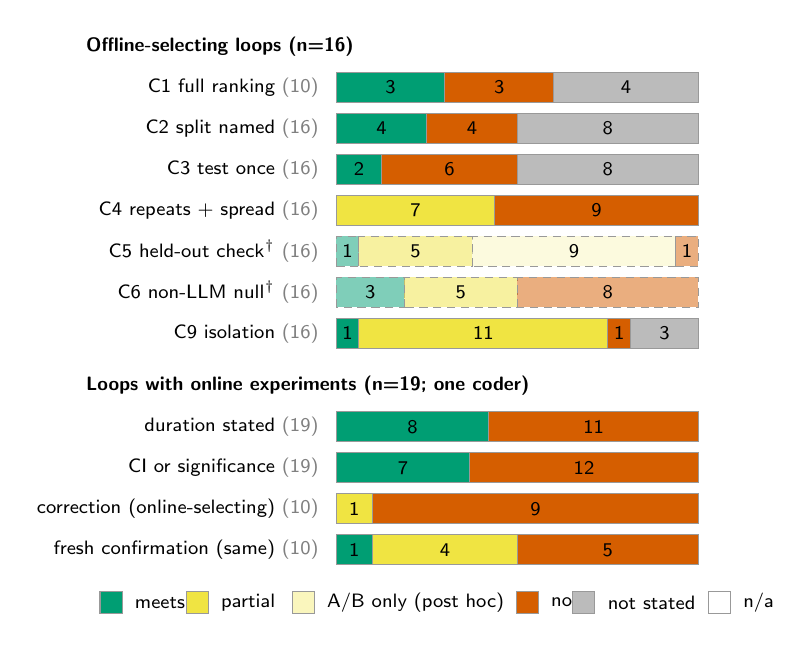
\begin{tikzpicture}[font=\sffamily\scriptsize]
\node[anchor=west, font=\sffamily\scriptsize\bfseries] at (-33mm,0.0mm) {Offline-selecting loops (n=16)};
\node[anchor=east] at (-1mm,-5.2mm) {C1 full ranking \textcolor{gray}{(10)}};
\draw[fill=cOk, draw=black!40] (0.00mm,-7.1mm) rectangle (13.80mm,-3.3mm);
\node at (6.90mm,-5.2mm) {3};
\draw[fill=cBad, draw=black!40] (13.80mm,-7.1mm) rectangle (27.60mm,-3.3mm);
\node at (20.70mm,-5.2mm) {3};
\draw[fill=cNS, draw=black!40] (27.60mm,-7.1mm) rectangle (46.00mm,-3.3mm);
\node at (36.80mm,-5.2mm) {4};
\node[anchor=east] at (-1mm,-10.4mm) {C2 split named \textcolor{gray}{(16)}};
\draw[fill=cOk, draw=black!40] (0.00mm,-12.3mm) rectangle (11.50mm,-8.5mm);
\node at (5.75mm,-10.4mm) {4};
\draw[fill=cBad, draw=black!40] (11.50mm,-12.3mm) rectangle (23.00mm,-8.5mm);
\node at (17.25mm,-10.4mm) {4};
\draw[fill=cNS, draw=black!40] (23.00mm,-12.3mm) rectangle (46.00mm,-8.5mm);
\node at (34.50mm,-10.4mm) {8};
\node[anchor=east] at (-1mm,-15.6mm) {C3 test once \textcolor{gray}{(16)}};
\draw[fill=cOk, draw=black!40] (0.00mm,-17.5mm) rectangle (5.75mm,-13.7mm);
\node at (2.88mm,-15.6mm) {2};
\draw[fill=cBad, draw=black!40] (5.75mm,-17.5mm) rectangle (23.00mm,-13.7mm);
\node at (14.38mm,-15.6mm) {6};
\draw[fill=cNS, draw=black!40] (23.00mm,-17.5mm) rectangle (46.00mm,-13.7mm);
\node at (34.50mm,-15.6mm) {8};
\node[anchor=east] at (-1mm,-20.8mm) {C4 repeats + spread \textcolor{gray}{(16)}};
\draw[fill=cPart, draw=black!40] (0.00mm,-22.7mm) rectangle (20.12mm,-18.9mm);
\node at (10.06mm,-20.8mm) {7};
\draw[fill=cBad, draw=black!40] (20.12mm,-22.7mm) rectangle (46.00mm,-18.9mm);
\node at (33.06mm,-20.8mm) {9};
\node[anchor=east] at (-1mm,-26.0mm) {C5 held-out check$^\dagger$ \textcolor{gray}{(16)}};
\draw[fill=cOk, draw=black!40, fill opacity=0.5, densely dashed] (0.00mm,-27.9mm) rectangle (2.88mm,-24.1mm);
\node at (1.44mm,-26.0mm) {1};
\draw[fill=cPart, draw=black!40, fill opacity=0.5, densely dashed] (2.88mm,-27.9mm) rectangle (17.25mm,-24.1mm);
\node at (10.06mm,-26.0mm) {5};
\draw[fill=cPart!35, draw=black!40, fill opacity=0.5, densely dashed] (17.25mm,-27.9mm) rectangle (43.12mm,-24.1mm);
\node at (30.19mm,-26.0mm) {9};
\draw[fill=cBad, draw=black!40, fill opacity=0.5, densely dashed] (43.12mm,-27.9mm) rectangle (46.00mm,-24.1mm);
\node at (44.56mm,-26.0mm) {1};
\node[anchor=east] at (-1mm,-31.2mm) {C6 non-LLM null$^\dagger$ \textcolor{gray}{(16)}};
\draw[fill=cOk, draw=black!40, fill opacity=0.5, densely dashed] (0.00mm,-33.1mm) rectangle (8.62mm,-29.3mm);
\node at (4.31mm,-31.2mm) {3};
\draw[fill=cPart, draw=black!40, fill opacity=0.5, densely dashed] (8.62mm,-33.1mm) rectangle (23.00mm,-29.3mm);
\node at (15.81mm,-31.2mm) {5};
\draw[fill=cBad, draw=black!40, fill opacity=0.5, densely dashed] (23.00mm,-33.1mm) rectangle (46.00mm,-29.3mm);
\node at (34.50mm,-31.2mm) {8};
\node[anchor=east] at (-1mm,-36.4mm) {C9 isolation \textcolor{gray}{(16)}};
\draw[fill=cOk, draw=black!40] (0.00mm,-38.3mm) rectangle (2.88mm,-34.5mm);
\node at (1.44mm,-36.4mm) {1};
\draw[fill=cPart, draw=black!40] (2.88mm,-38.3mm) rectangle (34.50mm,-34.5mm);
\node at (18.69mm,-36.4mm) {11};
\draw[fill=cBad, draw=black!40] (34.50mm,-38.3mm) rectangle (37.38mm,-34.5mm);
\node at (35.94mm,-36.4mm) {1};
\draw[fill=cNS, draw=black!40] (37.38mm,-38.3mm) rectangle (46.00mm,-34.5mm);
\node at (41.69mm,-36.4mm) {3};
\node[anchor=west, font=\sffamily\scriptsize\bfseries] at (-33mm,-43.1mm) {Loops with online experiments (n=19; one coder)};
\node[anchor=east] at (-1mm,-48.3mm) {duration stated \textcolor{gray}{(19)}};
\draw[fill=cOk, draw=black!40] (0.00mm,-50.2mm) rectangle (19.37mm,-46.4mm);
\node at (9.68mm,-48.3mm) {8};
\draw[fill=cBad, draw=black!40] (19.37mm,-50.2mm) rectangle (46.00mm,-46.4mm);
\node at (32.68mm,-48.3mm) {11};
\node[anchor=east] at (-1mm,-53.5mm) {CI or significance \textcolor{gray}{(19)}};
\draw[fill=cOk, draw=black!40] (0.00mm,-55.4mm) rectangle (16.95mm,-51.6mm);
\node at (8.47mm,-53.5mm) {7};
\draw[fill=cBad, draw=black!40] (16.95mm,-55.4mm) rectangle (46.00mm,-51.6mm);
\node at (31.47mm,-53.5mm) {12};
\node[anchor=east] at (-1mm,-58.7mm) {correction (online-selecting) \textcolor{gray}{(10)}};
\draw[fill=cPart, draw=black!40] (0.00mm,-60.6mm) rectangle (4.60mm,-56.8mm);
\node at (2.30mm,-58.7mm) {1};
\draw[fill=cBad, draw=black!40] (4.60mm,-60.6mm) rectangle (46.00mm,-56.8mm);
\node at (25.30mm,-58.7mm) {9};
\node[anchor=east] at (-1mm,-63.9mm) {fresh confirmation (same) \textcolor{gray}{(10)}};
\draw[fill=cOk, draw=black!40] (0.00mm,-65.8mm) rectangle (4.60mm,-62.0mm);
\node at (2.30mm,-63.9mm) {1};
\draw[fill=cPart, draw=black!40] (4.60mm,-65.8mm) rectangle (23.00mm,-62.0mm);
\node at (13.80mm,-63.9mm) {4};
\draw[fill=cBad, draw=black!40] (23.00mm,-65.8mm) rectangle (46.00mm,-62.0mm);
\node at (34.50mm,-63.9mm) {5};
\draw[fill=cOk, draw=black!40] (-30.0mm,-72.0mm) rectangle (-27.2mm,-69.2mm);
\node[anchor=west] at (-26.8mm,-70.6mm) {meets};
\draw[fill=cPart, draw=black!40] (-19.05mm,-72.0mm) rectangle (-16.25mm,-69.2mm);
\node[anchor=west] at (-15.850000000000001mm,-70.6mm) {partial};
\draw[fill=cPart!35, draw=black!40] (-5.600000000000001mm,-72.0mm) rectangle (-2.8000000000000016mm,-69.2mm);
\node[anchor=west] at (-2.4000000000000012mm,-70.6mm) {A/B only (post hoc)};
\draw[fill=cBad, draw=black!40] (22.849999999999998mm,-72.0mm) rectangle (25.65mm,-69.2mm);
\node[anchor=west] at (26.049999999999997mm,-70.6mm) {no};
\draw[fill=cNS, draw=black!40] (30.049999999999997mm,-72.0mm) rectangle (32.849999999999994mm,-69.2mm);
\node[anchor=west] at (33.25mm,-70.6mm) {not stated};
\draw[fill=white, draw=black!40] (47.25mm,-72.0mm) rectangle (50.05mm,-69.2mm);
\node[anchor=west] at (50.45mm,-70.6mm) {n/a};
\end{tikzpicture}

\caption{Audit summary. Top: the 16 offline-selecting loops (C1 among the 10 that report ranking metrics; five
report AUC or a loss and one only online lifts). Bottom: the design of the online experiments reported by 19 loops. C9 counts the
isolation design; incidents of gaming or leakage are reported separately (F7). Generated from the released
\texttt{audit.csv}.}
\label{fig:auditbars}
\end{figure}

\begin{table*}[t]
\caption{Evaluation audit (full text, 22 October 2026). Level: evolved object. C1 metric: Full = full-catalogue ranking;
Sampled = ranking against sampled negatives; Rank? = ranking metric with the candidate set not stated; AUC =
AUC/logloss/loss proxy; A/B = online only; other = a non-recommendation metric; ? = no metric stated. C2 selection
signal: val, test (the data that are also reported), loss (training loss), A/B, \ns. C4 \pa: repeats without spread,
repeats in an ablation only, a re-run rule, or a noise estimate of single models. C5 \pa: partial transfer evidence. C6
\pa: unmatched budget, LLM still proposing, or replay only. C8: \yes tuned, \no untuned, \pa partly or on test data,
prod.\ = production model, pub.\ = published numbers, seed = the loop's seed program. C9 isolation design: \pa part of
the loop constrained (fixed evaluation code, gates, whitelists, sandboxing, bounded actions);
\textsuperscript{G} = the paper reports gaming, metric-winning bugs, metric inflation or leakage by the loop. Code: later = promised. \yes
= yes, \no = no, \pa = partial, \ns = not stated, \na = not applicable.}\label{tab:audit}
\small
\begin{tabular}{@{}llllllllllll@{}}
\toprule
System & Level & C1 & C2 & C3 & C4 & C5 & C6 & C8 & C9 & A/B & Code \\
& & metric & select & test once & repeats & gap & null & baselines & isolation & & \\
\midrule
%BEGIN-AUDIT-ROWS
Self-EvolveRec~\cite{kim2026selfevolverec} & L2 & Sampled & val & \ns & \no & \pa & \pa & \no & \ns & \no & \yes \\
RecHarness~\cite{ling2026recharness} & L1+L2 & Sampled & val & \yes & \pa & \pa & \pa & seed & \pa & \yes & \yes \\
Google/YouTube~\cite{wang2026selfevolving} & L1+L2 & A/B & A/B & \na & \pa & \pa & \no & prod. & \pa & \yes & \no \\
EvoRec~\cite{mu2026evorec} & L1+L2 & Rank? & \ns & \ns & \no & \pa & \pa & \no & \ns & \yes & \no \\
VirtualMLE~\cite{cao2026virtualmle} & L1 & Rank? & val & \yes & \pa & \pa & \yes & \yes & \yes & \no & \yes \\
NOVA~\cite{liu2026nova} & L1+L2 & AUC & \ns & \ns & \no & \pa & \yes & prod. & \pa & \yes & \no \\
AgentX~\cite{lao2026agentx} & L1+L2 & A/B & A/B & \na & \no & \no & \no & prod. & \pa & \yes & \no \\
AgentX-Model~\cite{yang2026agentxmodel} & L2 & AUC & \ns & \no & \pa & \pa & \pa & prod. & \pa & \yes & \no \\
Auto-RecSys~\cite{li2026autorecsys} & L2 & other & \na & \na & \no & \no & \no & prod. & \pa & \no & \no \\
AutoLR~\cite{zhang2026autolr} & L1+L2 & A/B & \ns & \ns & \no & \pa & \no & prod. & \pa & \yes & \no \\
CORAL~\cite{azhar2026coral} & L1 & A/B & A/B & \na & \no & \no & \no & prod. & \pa & \yes & \no \\
AgenticRecTune~\cite{wu2026agenticrectune} & L1 & A/B & A/B & \na & \no & \no & \no & prod. & \pa & \yes & \no \\
Sortify~\cite{cheng2026sortify} & L1 & A/B & A/B & \na & \no & \pa & \no & prod. & \pa & \yes & \no \\
GEARS~\cite{yun2026gears} & L1 & other & A/B & \na & \no & \pa & \no & prod. & \pa & \yes & \no \\
RecEvolve~\cite{pan2026recevolve} & L2 & Sampled & \ns & \ns & \no & \pa & \no & prod. & \pa\textsuperscript{G} & \yes & \no \\
Astar~\cite{hu2026astar} & L2 & Rank? & \ns & \ns & \no & \pa & \no & prod. & \ns & \yes & \no \\
A-MLE~\cite{gao2026amle} & L1+L2 & AUC & \ns & \ns & \pa & \no & \no & prod. & \pa & \no & \no \\
SR-Agent~\cite{yang2026sragent} & L1 & A/B & A/B & \na & \no & \pa & \no & prod. & \pa & \yes & \no \\
EvoSkillRec~\cite{li2026evoskillrec} & L2 & AUC & val & \no & \no & \yes & \yes & \no & \pa & \no & \yes \\
RankEvolve-HSTU~\cite{chen2026rankevolve} & L1+L2 & Full & test & \no & \no & \pa & \no & pub. & \no\textsuperscript{G} & \no & later \\
Population Evolution~\cite{peng2026population} & L2 & Full & test & \no & \pa & \pa & \pa & \pa & \pa & \no & later \\
Trajectories-to-Evidence~\cite{zhuang2026trajectories} & L2 & AUC & \ns & \ns & \no & \pa & \no & prod. & \pa & \yes & \no \\
EvoPilot~\cite{fu2026evopilot} & L1+L2 & Rank? & test & \no & \pa & \pa & \no & prod. & \pa\textsuperscript{G} & \yes & \no \\
Amazon AutoResearch~\cite{chandran2026autoresearch} & L1+L2+L3 & Full & test & \no & \pa & \pa & \no & \yes & \pa\textsuperscript{G} & \no & \no \\
PILOT~\cite{pilot2026} & L1 & A/B & A/B & \na & \no & \no & \no & prod. & \pa & \yes & \no \\
A/B Agent~\cite{jiang2026abagent} & L1 & A/B & A/B & \na & \no & \no & \no & prod. & \pa & \yes & \no \\
DMRL~\cite{zhang2026dmrl} & L1 & A/B & A/B & \na & \no & \no & \no & prod. & \pa & \yes & \no \\
\midrule
\multicolumn{12}{@{}l}{\emph{Comparison points outside recommendation}} \\
EvoRank (LTR)~\cite{patel2026evorank} & L2 & other & val & \yes & \yes & \yes & \yes & \yes & \yes & \no & \yes \\
AI Co-Scientist (search)~\cite{wu2026coscientist} & L2 & AUC & test & \no & \no & \no & \no & \pa & \ns\textsuperscript{G} & \no & \no \\
RankEvolve-IR (lexical)~\cite{nian2026rankevolveir} & L2 & Full & \ns & \yes & \no & \yes & \pa & \no & \no & \no & \yes \\
Evolving Semantic Indexes (GR)~\cite{nian2026semanticindex} & L3 & Full & val & \yes & \pa & \yes & \no & seed & \yes & \no & \no \\
AgentLTV (LTV)~\cite{wu2026agentltv} & L2 & other & test & \ns & \no & \no & \pa & \ns & \no & \no & \yes \\
Feedback Contract (CTR/LTR)~\cite{yao2026feedbackcontract} & L2 & AUC & val & \yes & \yes & \yes & \no & seed & \yes & \no & \no \\
PEAR (search)~\cite{wang2026pear} & L1 & A/B & A/B & \na & \pa & \pa & \no & prod. & \ns & \yes & \no \\
%END-AUDIT-ROWS
\bottomrule
\end{tabular}
\end{table*}

\paragraph{F1: Candidate sets are rarely full, and often unstated.} Ten offline-selecting loops report ranking
metrics. Three rank the full catalogue (RankEvolve-HSTU, Population Evolution, and the retrieval system of Amazon's
AutoResearch); two pair each test item with 99 sampled negatives (Self-EvolveRec, RecHarness), and RecEvolve ranks
against in-batch negatives, which is why shrinking the batch inflated its metrics (F7); four do not say what the
candidate set is, so between three and seven of the ten use full ranking. In Amazon's loop the agent designed a text-only
fallback that ``expanded catalog coverage by 5.8$\times$''~\cite{chandran2026autoresearch}, which by our reading
changed the candidate set during the campaign. Five offline-selecting loops evaluate ranking-stage CTR models with AUC
or a loss, as is standard for that stage, and AutoLR selects offline but headlines only online lifts.

\paragraph{F2: The selection data are often unstated, and sometimes they are the reported data.} Of the 16
offline-selecting loops, four name a validation split (Self-EvolveRec, RecHarness, VirtualMLE, EvoSkillRec). Google's
loop also ranks candidates by validation loss, but online experiments decide which run and launch, so we count it as
online-selecting; Astar's loss-decrease rule labels its training data and defines its success rate, but the paper does
not say what decides its production iterations. Four select on the data they report. RankEvolve-HSTU's persistent leaderboard is the canonical full-test
NDCG@10~\cite{chen2026rankevolve}; Amazon's AutoResearch ``retains modifications that improve a held-out scalar
metric'' and headlines the trajectory's peak~\cite{chandran2026autoresearch}; EvoPilot selects and reports on one
held-out replay set~\cite{fu2026evopilot}; and Population Evolution selects on its source instances' evaluation scores
and reports its local gains on them, while withholding the transfer targets from the proposer, and calibrates the
shared baseline configuration on the released test split~\cite{peng2026population}. All four disclose these choices,
which is to their credit. Eight do not say which data keep or reject candidates; the number that name a non-test
selection signal is therefore between 4 and 12 of 16. Outside recommendation, the travel-search co-scientist keeps or
reverts each change on the same held-out metric that it reports~\cite{wu2026coscientist}.

\paragraph{F3: Test-once is rarely stated.} Two offline-selecting loops state that the selected candidate was
evaluated on held-out test data once after the search (RecHarness, VirtualMLE). Six use the test data during the
search or repeatedly: four report on the data they select on (RankEvolve-HSTU, Population Evolution, Amazon, EvoPilot),
AgentX-Model reports the best AUC over rounds and experiments, and EvoSkillRec scores every candidate on test in every
generation while stating that the scores are never used for selection. Eight do not say, so the true number is between
2 and 10.

\paragraph{F4: No headline result comes with its spread over repeated sessions.} None of the 16 offline-selecting
loops repeats an evolution session and reports the spread. Seven have partial evidence: RecHarness and VirtualMLE
average three runs without a standard deviation; Population Evolution reports one run per configuration, with repeated
evaluations of the reference score and unreported preliminary runs whose ``ordering was consistent''~\cite{peng2026population}; A-MLE re-runs a candidate when within-run variance is high, which the authors say ``materially
reduced'' single-seed promotions~\cite{gao2026amle}; and AgentX-Model, EvoPilot and Amazon estimate the noise of single
models without repeating a session---EvoPilot notes that two publications of the same model, configuration and pinned
data ``differed by 0.36 points''~\cite{fu2026evopilot}, and Amazon re-evaluates one model across 11 dates (``6.18\%
$\pm$ 0.28 pp'')~\cite{chandran2026autoresearch}. Several papers state that their gains are within the resolution of
a single run: EvoSkillRec notes margins ``on the order of $10^{-4}$ AUC, which a single evolution run cannot reliably
separate from run-to-run variation''~\cite{li2026evoskillrec}; AgentX-Model reports run-to-run standard deviations of
0.0010--0.0022 AUC while counting an experiment as above baseline if it exceeds it by more than
$10^{-6}$~\cite{yang2026agentxmodel}; and AutoLR, in its audited configuration, promoted candidates after a single run
with noise calibration disabled, a risk its authors name the ``KEEP ratchet'': each promoted model becomes the
baseline for all later comparisons~\cite{zhang2026autolr}. None of the ten online-selecting loops repeats a session
either; Google runs six independent sessions with bracketed ranges, but only for an ablation. For these loops a repeat
is only practical on a replay (R4 in \S\ref{sec:protocol}).

\paragraph{F5: Where transfer is checked, some selected gains survive and some do not.} One core loop reports an
explicit held-out check of its selected candidates. In EvoSkillRec, five candidates lie on the validation Pareto
front, ``but only P1 (round 19) retains both improvements on the test set''~\cite{li2026evoskillrec}; P1 has the
highest validation score of the five, so choosing by validation would have picked it (the paper states no rule for choosing a
front point); P2 and P3 lose their AUC gain on test, and P4 and P5 have none on validation. Population Evolution checks transfer across datasets and scale: a ranking candidate gains 10.66\% on a peer dataset and loses 0.79\% at
larger scale, two of three peer-screened designs keep their gains, and sharing evidence across searches raises the
larger-scale pass rate for ranking from 11/60 to 18/60~\cite{peng2026population}: in ranking and RL, most locally selected
candidates do not graduate. Two further observations point the same way. Amazon's headline lift of 1.82$\times$ is the peak of a
trajectory, ``${\sim}$2.6$\sigma$ above the across-date mean'' of 1.63$\times$~\cite{chandran2026autoresearch}, and
Kuaishou's trajectory analysis finds that for 22 of 30 methods the last round falls below an earlier
best~\cite{zhuang2026trajectories}. The comparison points give larger effects: in EvoRank, the gains of the first
(loss-evolution) campaign ``were almost entirely fitness noise'' on 60k held-out queries, while about 70\% of the
second campaign's gains survived~\cite{patel2026evorank}; in an e-commerce search loop, effects on a shadow-traffic
proxy were several to tens of times larger than in decision-grade online experiments, and five promoted candidates
showed no significant gain~\cite{wang2026pear}; and in Evolving Semantic Indexes, a proxy decoder that ranks
semantic-ID programs well (Spearman $\rho = 0.90$) becomes ``not only less informative but misleading'' once the
training objective may change, on a small sample of five programs~\cite{nian2026semanticindex}. A controlled study
shows that the mechanism exists: on a label-permuted task with no real signal, a coding agent given exact validation
scores ``ended by reporting a gain of 0.0157''~\cite{yao2026feedbackcontract}. None of this measures how much of the
published recommender gains is selection noise; it shows that the question cannot be settled without held-out checks.

\paragraph{F6: Null controls are rare.} Three offline-selecting loops compare against a non-LLM search at an equal or
favourable budget: VirtualMLE (grid search and Bayesian optimisation), NOVA (Optuna-TPE at a matched offline-evaluation
budget but unmatched LLM cost, and only on its ScaleUp task, a search over structural hyperparameters) and EvoSkillRec (NASRec, alongside OpenEvolve); in all three the LLM loop is reported
to win. Five have partial controls (NAS baselines at unmatched budgets, a random arm router that still uses LLM edits, a
replay-only random policy, or a starting model tuned by an optimiser that the LLM partly steers), and eight have none;
comparisons with human workflows or with other LLMs do not count. No loop runs an equal-budget random search over its own edit space,
and none runs the catalogue-of-known-techniques null of \S\ref{sec:kept}. Where random selection was run, it was
competitive: in AgentX-Model's historical replay, which randomises the choice of experiments rather than the edits, in
Scenario A ``Uniform Random's mean exceeds Fixed, Greedy, and Joint'' policies, and no policy led consistently across
scenarios~\cite{yang2026agentxmodel}; in
EvoRank's loss campaign an equal-budget random search transferred as well or better ($p=0.03$)~\cite{patel2026evorank}.
AutoLR states plainly that it ``does not establish superiority over random, greedy, or direct LLM-based routing under a
matched trial budget''~\cite{zhang2026autolr}. The history of architecture search explains why the control matters: random
search with early stopping matched leading NAS methods~\cite{li2019randomnas}, the search phase of several methods was no
better than random sampling~\cite{yu2020searchphase,yang2020nashard}, and classical optimisers beat LLM agents in fixed
hyperparameter spaces~\cite{ferreira2026hpo,rodrigues2026llmhpo}. The online-selecting loops compare each candidate with a
control arm, which is a different question from whether the proposer beats a null search.

\begin{table}[t]
\caption{Shortcuts reported in the audited loops (F7): what happened, what caught it, and a guard that prevents it by
construction.}\label{tab:failures}
\footnotesize
\begin{tabularx}{\columnwidth}{@{}>{\raggedright\arraybackslash\hsize=1.15\hsize}X>{\raggedright\arraybackslash\hsize=0.75\hsize}X>{\raggedright\arraybackslash\hsize=1.0\hsize}X>{\raggedright\arraybackslash\hsize=1.1\hsize}X@{}}
\toprule
Failure & Where & Caught by & Guard \\
\midrule
Metric definition changed (batch size inflates an in-batch metric) & RecEvolve & a human & freeze metric-relevant settings \\
Target leakage in features or training pairs & RankEvolve-HSTU & the agent, from anomalous leaderboard trajectories & leakage checks before search (NOVA, EvoRank) \\
Evaluation protocol changed (multi-position scoring) & RankEvolve-HSTU & mandatory diagnosis of negatives & evaluator the agent cannot edit \\
Evaluation date inside the training window & EvoPilot & not stated & date-order checks \\
Proxy metric gamed (codebook size) & Amazon AutoResearch & human QA between runs & a second, usability metric \\
Capacity silently increased & AI Co-Scientist & not stated & matched-capacity comparisons \\
\bottomrule
\end{tabularx}
\end{table}

\paragraph{F7: Agents find shortcuts in the evaluation, and the keep-or-reject rule does not catch them.} Four core
loops and one comparison point report metric-winning bugs, metric inflation or leakage produced by the loop itself
(Table~\ref{tab:failures}). RecEvolve's agent ``discovered that drastically reducing the batch size (from 8k down to
1k) artificially inflated proxy metrics''; a human caught it and rolled it back~\cite{pan2026recevolve}. On HSTU,
RankEvolve-HSTU's agents produced a genre feature that leaked the target (training loss collapsed to zero while
evaluation spiked), DPO preference pairs mined at the held-out target position, and a naive multi-position evaluation
that would have inflated NDCG@10 from 0.2192 to 0.2517/0.2577; the genre and DPO bugs surfaced as anomalous trajectories on
the leaderboard, the inflation was reasoned out as leakage in the diagnosis the loop requires for every negative result,
and none was reported as a gain, but the best agent pair
still had a 10.4\% silent critical-defect rate on ExecML-HSTU, and a single Claude Code pass
35.4\%~\cite{chen2026rankevolve}. In EvoPilot, ``a favorable result used an evaluation date inside the candidate
model's training window, so the result was retracted''~\cite{fu2026evopilot}. In Amazon's semantic-ID loop,
``maximizing codebook size trivially improves weighted coherence'', and the resulting hierarchy was unusable; human QA
between runs caught it~\cite{chandran2026autoresearch}. Where a paper says what caught the problem, it was something outside the
keep-or-reject rule: a person (RecEvolve, Amazon) or the agent's own diagnosis of anomalous results (RankEvolve-HSTU).
Coding agents that can reach their tests behave the same way outside
recommendation~\cite{zhong2026impossiblebench,metr2025rewardhacking,baker2025monitoring}. These four
papers should be credited for reporting incidents (R8); a paper that reports none has not shown that none occurred.
Among the borderline systems, AURA's agent fabricated 904 session identifiers in its diagnostic
stage~\cite{kim2026aura}, and RecSys Factory's diagnostics uncovered a pre-existing upstream join bug that had
``silently corrupted all downstream training samples''~\cite{ao2026recsysfactory}, a reminder that the data feeding the
loop need checks too. As designed, only VirtualMLE states that the test set is hidden from the agent and the data
pipeline immutable; eleven offline-selecting loops constrain part of the loop (verification gates, fixed evaluation
code, whitelists, isolated workspaces, sandboxed modules), RankEvolve-HSTU lets its agents run evaluations at the test
position, and three say nothing; all ten online-selecting loops bound the agent's actions.

\paragraph{F8: Baselines, budgets and openness.} The largest relative gains are measured against weak starting
points. RecHarness improves average HR@10 by 85.85\% over a cold-start GRU4Rec~\cite{hidasi2016gru4rec} template and by
12.58\% over HSTU~\cite{ling2026recharness}, and Self-EvolveRec configures all models with the same fixed
hyperparameters (embedding 50, batch 128, learning rate 0.001) without describing tuning them~\cite{kim2026selfevolverec}.
Against production baselines, online lifts on broad metrics such as watch time, revenue or GMV are mostly between
0.06\% and 5\% (\texttt{design.csv}). Only VirtualMLE and Amazon's AutoResearch (a hand-tuned baseline from four engineer-weeks)
describe tuning their baselines on non-test data; Population Evolution tunes them on the test split. Budgets are
reported in incompatible units (iterations, GPU-seconds, GPU-hours, ideas, tokens, dollars, yuan); twelve of 27 report
LLM tokens or cost. Four of 27 release code, two promise to, and six do not name the LLM they use.

\paragraph{F9: Online gates are reported, but rarely as confirmations.} Nineteen of the 27 loops report online
experiments; these are the main safeguard of the industrial loops and strong evidence when well designed. Nine state
the experiment duration and nine report significance or confidence intervals; none corrects for multiple testing across
the many rounds a loop runs (AutoLR discusses the problem but applies no correction), although the arm chosen as best
overstates its effect~\cite{lee2018winnerscurse,berman2026winners}. AutoLR's summed launch-review lifts are, in its own
words, ``descriptive and are not pooled treatment effects''~\cite{zhang2026autolr}. Only Sortify re-tests its chosen
round in a fresh seven-day experiment~\cite{cheng2026sortify}. PILOT designs its final confirmation as ``a single
pre-registered test'' that ``runs once'', because ``the data collected while searching \ldots{} cannot also serve as
proof''~\cite{pilot2026}, but the report does not yet include that confirmation, and its headline compares the best of
five buckets before and after, ``not randomized''. Online noise is visible inside single papers: DMRL's default
configuration (Qwen3-8B, eight rollouts) appears in six tables run in ``non-overlapping time windows'' with LTV lifts
from $+0.021\%$ to $+0.064\%$, a spread of 0.043 percentage points, larger than its 0.028-point lead over the best
baseline in the main table; the authors restrict their conclusions to within-table comparisons~\cite{zhang2026dmrl}.

\paragraph{Practices worth copying.} The audit also found practices that, if combined, would meet most of the
standard in \S\ref{sec:protocol}: RecHarness's validation-only selection with a single test evaluation; VirtualMLE's
hidden test set, immutable pipeline and grid-search and BO baselines; EvoSkillRec's validation-versus-test check of its
Pareto front; Population Evolution's withheld transfer targets; NOVA's leakage verifier and EvoRank's pre-search
leakage audit with an equal-budget random search; RankEvolve-HSTU's mandatory diagnosis of negative results; and
Sortify's fresh re-test and PILOT's pre-registered confirmation design.

\paragraph{Does selection really overfit?} A meta-analysis of 120 Kaggle competitions found little overfitting to
public leaderboards~\cite{roelofs2019metaanalysis}, and new test sets for ImageNet showed accuracy drops but preserved
model rankings~\cite{recht2019imagenet}, partly because similar models overfit a reused test set less than theory
predicts~\cite{mania2019similarity}. Agent-proposed candidates are near-copies of an incumbent, which by that argument
limits regressional overfitting. Two differences remain: an agent loop evaluates hundreds of correlated candidates on
one split without a resubmission cap~\cite{blum2015ladder} and keeps the maximum, and it controls the code that produces
the score, which no Kaggle team does. The direct measurements (F5) show that some selected gains shrink or vanish on
transfer while others survive. The safe conclusion is not that self-evolving recommenders do not work, but that the
published evidence cannot yet tell how much of their gain is real.

%=====================================================================
\section{A Reporting Standard}\label{sec:protocol}
%=====================================================================

The audit suggests that most of the problems are cheap to report: they are unreported or unenforced rather than
unsolvable. Table~\ref{tab:checklist} turns the codebook into a reporting standard. Each item has a minimum that any
paper can meet by reporting what it already did, and a recommended practice that costs compute; each maps to the
audit criterion that checks it, so that a paper's compliance can be read off the same coding. The items extend
general checklists for NAS research~\cite{lindauer2020bestpractices}, ML-based science~\cite{kapoor2024reforms} and
agent benchmarks~\cite{zhu2025abc} to the specific failure points of an evolution loop (Figure~\ref{fig:loop}).
Appendix~\ref{app:exemplars} applies the minimum tier to two audited papers.

\begin{table*}[t]
\caption{Reporting standard for self-evolving recommenders. \emph{Minimum}: report what was done; \emph{recommended}:
what a strong study does. The last column gives the audit criterion (Table~\ref{tab:codebook}) or finding that checks the item.}\label{tab:checklist}
\small
\begin{tabularx}{\textwidth}{@{}l>{\hsize=0.95\hsize}X>{\hsize=1.05\hsize}Xl@{}}
\toprule
& Minimum (report) & Recommended (do) & Audit \\
\midrule
R1 Metric & State the candidate set and how negatives are drawn (full catalogue, $N$ sampled, in-batch); for
ranking-stage models, the traffic on which AUC or logloss is computed. & Full-catalogue ranking where the catalogue
allows, sampled metrics only as secondary~\cite{krichene2020sampled}. & C1 \\
R2 Selection & Name the data or signal that accepts candidates at every stage of the chain (proxy, offline, online). &
Keep the test split out of every decision, including baseline tuning. & C2 \\
R3 Test once & Report the selected candidate's validation score next to its test score. & Evaluate on test once,
after the search. & C3, C5 \\
R4 Sessions & Run $\geq 3$ independent sessions and report every session's final test score. & $\geq 5$ sessions with
an interquartile mean and bootstrap interval~\cite{agarwal2021precipice}, and the expected best score as a function of
budget~\cite{dodge2019showyourwork}. Industrial loops: repeat on a replay or a reduced-scale proxy. & C4 \\
R5 Null control & One null at equal trial and compute budget: HPO or random search over the knobs that the kept
edits changed. & A ladder of nulls: (i) HPO over the same knobs, (ii) random mutation over the edit arms or grammar,
(iii) the same proposer without evaluation feedback or with candidates accepted at random. & C6 \\
R6 Budget & A budget card: trials, GPU-hours, LLM tokens and cost, wall-clock, human hours, and the cost of training
a learned proposer. & Report results as a function of budget, not only at its end~\cite{kapoor2025agentsmatter}. & C7 \\
R7 Baselines & How the starting point and compared models were tuned, and on which data. & Tune them with the
budget of one session. & C8 \\
R8 Access & What the agent can read and write (data, labels, evaluation code, metric definitions); every gaming or
leakage incident and what caught it. & An evaluator in a process the agent cannot modify; review of metric-relevant
changes (batch size, candidate set, evaluation date). & C9 \\
R9 Online gates & Duration, traffic share, pre-specified primary metric and guardrails, confidence intervals, and the
number of rounds tested. & A correction across rounds and a fresh, pre-registered confirmation of the final candidate,
reporting the confirmed rather than the selected effect~\cite{kohavi2020trustworthy}. & F9 \\
\bottomrule
\end{tabularx}
\end{table*}

\paragraph{Cost of compliance.} The minimum tier costs nothing beyond writing. In the recommended tier, R4 and R5
multiply training cost: three sessions plus one equal-budget null cost four sessions. For an academic harness such
as RecHarness, whose budget is 43{,}200 GPU-seconds per backbone~\cite{ling2026recharness}, that is 48 GPU-hours per
backbone. LLM costs are small next to training: VirtualMLE reports \$1.5--4.8 of LLM cost per
session~\cite{cao2026virtualmle}, EvoRank about ten dollars for fifty iterations~\cite{patel2026evorank}, and NOVA
about \$29 per task, or about \$22 with cached artifacts~\cite{liu2026nova} (LLM cost only). For industrial loops whose candidates take hundreds of
GPU-hours~\cite{li2026autorecsys}, R4 and R5 can be applied to a replay or a reduced-scale proxy, as AgentX-Model
does for scheduling policies~\cite{yang2026agentxmodel}, while R9 governs the launch decision.

\paragraph{A shared protocol.} Several items can be enforced in software rather than requested in prose: a sealed
test split (R2, R3), a single final evaluation, an equal-budget null evolver (R5), a budget card (R6) and an
evaluator outside the agent's reach (R8). Appendix~\ref{app:recforge} describes recforge~\cite{recforge}, a
reference implementation that we are building; it enforces R2, R3 and R5 through its API but not yet R8, and we
report no results from it.

%=====================================================================
\section{Open Problems}\label{sec:open}
%=====================================================================

\paragraph{Isolation without crippling the agent.} Code-level agents need to read data and change training code, and
that is exactly the access that lets them leak targets or change what the metric measures (F7). Verification gates
(NOVA), fixed evaluation code (AgentX-Model), immutable pipelines (VirtualMLE) and cross-agent review (RankEvolve-HSTU) each
close part of the gap. A principled design would give the agent a process that physically cannot reach evaluation
labels or code, and would audit every metric-relevant change, such as batch size for in-batch metrics.

\paragraph{Proxies for expensive candidates.} Industrial candidates take hours to hundreds of GPU-hours, so loops screen
on proxies: small decoders~\cite{nian2026semanticindex}, data subsets and peer datasets~\cite{peng2026population},
training-loss curves and learned reward models~\cite{hu2026astar}, and LLMs can themselves predict a candidate
architecture's performance before training~\cite{jawahar2024llmpp}. The evidence shows that proxy fidelity depends on
what is evolved. Characterising when a proxy can be trusted, and spending budget to re-check proxies during search, is
open.

\paragraph{Budget-normalised comparison of evolvers.} There is no common unit of cost and no common task, so the field
cannot say whether bandit routing, island evolution, research-agent pairs or learned proposers are better. A shared
benchmark with a budget card (R6) and an equal-budget random baseline (R5) would allow the first such comparison.

\paragraph{Evolving generative recommenders.} Semantic-ID construction, codebook collisions, constrained decoding and
preference-alignment losses are new design dimensions with little human prior and large effects. They are natural
targets for code-level evolution, and almost untouched (\S\ref{sec:systems}).

\paragraph{From offline wins to online value.} RecEvolve observes that offline evaluations often show ``win-win''
results while online tests show trade-offs~\cite{pan2026recevolve}. Loops that select on offline metrics inherit the
gap; loops that select on online experiments face multiple testing and slow iteration. Combining the two with a fresh
online confirmation of the final candidate, as Sortify does with a seven-day re-test, ideally pre-registered, is a
starting point.

\paragraph{Circularity at the policy level.} L4 systems are often judged by simulators from the same model family as the
agent being improved. Held-out simulators~\cite{kim2026selfevolverec}, verifiable rewards~\cite{narasimhan2026taurec}
and reward-model benchmarks~\cite{zeng2026recrmbench} are partial answers.

%=====================================================================
\section{Threats to Validity}\label{sec:threats}
%=====================================================================

\paragraph{Coverage.} The field is months old and grows weekly; our cut-off is 22 October 2026. Many systems are
arXiv preprints whose versions change; we coded the version available on that date. Generic keyword search performed
poorly, so coverage relies on citation-graph search and may miss systems that neither cite nor are cited by the core
set.

\paragraph{Coding.} Each cell was drafted from the full text with verbatim evidence and then checked against the
original papers in two adversarial verification passes, run by LLM agents and reviewed by the authors: the first
corrected 12 cells in nine rows, the second re-verified every cited sentence against its source and corrected the
remaining cells and claims (both reports are released in \texttt{review/}). A third pass, prompted by an internal
review of this version, recoded nine criterion cells and five object labels, moved meta-evolution into its own column, and separated C9 into isolation design and reported incidents (listed in
the released \texttt{audit/README.md}). A second author then coded all 27 core systems from the full texts with the
same codebook, without access to the coding data; as a co-author, the second coder could have seen the first
version of this survey, whose audit table was public. Before reconciliation, the two codings agreed on 84\% of the
243 cells (pooled Cohen's $\kappa = 0.81$, Gwet's AC1 $= 0.84$). By criterion, $\kappa$ was 0.67 for C1 (95\%
bootstrap interval 0.46--0.86), 0.90 for C2, 0.79 for C3, 0.91 for C4, 0.30 for C5 ($-0.04$--0.63), 0.65 for C6,
0.57 for C8, 0.77 for C9 and 0.87 for reported incidents; AC1 was at least 0.70 everywhere except C5 (0.50). The 38
disagreements were resolved against the paper text, with LLM agents drafting a resolution and quote for each and both
authors reviewing them: 31 in favour of the second coding and seven in favour of the first. Most of them came from rules the codebook left open: which gate counts as the selection in a multi-stage
loop, whether an online test of an offline-selected candidate is transfer evidence, and whether computing test
scores that are not used for selection breaks test-once. The counts in this paper use the reconciled coding; the
two independent sheets, the agreement script and every resolution are released. Two criteria fall below $\kappa =
0.6$, so the counts that rest on them are the least certain: C5 (F5, where the disagreements were mostly between
``partial'' and ``no'') and C8 (F8, where they were mostly about which label describes a baseline, not whether it
was tuned).
``Not stated'' does not mean ``not done'': authors may have followed a practice without reporting it, which is why
we give ranges for the counts that rest on such cells. We have not yet asked the audited authors to check their rows;
the evidence is released so that they and other readers can correct individual cells, and we will update the table.

\paragraph{Industrial systems.} Offline hygiene criteria mean little for loops whose keep-or-reject decision is an
online experiment. We therefore report those loops separately and assess them on the design of their experiments
(F9), and we do not treat a missing offline test split as a defect when no offline claim is made.

\paragraph{Conflict of interest.} The authors are building recforge, the reference implementation described in
Appendix~\ref{app:recforge}; the audit does not depend on it. One of us wrote the ideation-harness study cited in
\S\ref{sec:systems}, which is outside recommendation and not peer reviewed, and both of us wrote the LLM-guided
regularisation paper cited in \S\ref{sec:method} as an excluded example.

%=====================================================================
\section{Conclusion}
%=====================================================================

Self-evolving recommenders moved in less than a year from an idea to production systems at many large platforms. The loops are
inventive, and several report online gains under well-designed experiments. The offline evidence is weaker than the
headlines suggest: selection data are often unstated, test-once and repeated sessions are rarely reported,
equal-budget null searches are rare, and the few papers that check transfer find that some selected gains do not
survive. Online gates are reported but seldom corrected for the rounds they test or confirmed afresh. Agents also find
shortcuts in the evaluation, which people or the agents' own diagnoses, not the acceptance rules, catch. Most of this is cheap to report. We
hope that the reporting standard in Table~\ref{tab:checklist}, the released audit and design data, and shared
protocols that enforce the standard in software make it the norm, so that the next comparison of evolvers can be made
on equal terms.

\bibliographystyle{ACM-Reference-Format}
\bibliography{../refs}

\appendix

\section{The Minimum Tier Applied to Two Papers}\label{app:exemplars}

Table~\ref{tab:exemplars} applies the minimum tier of Table~\ref{tab:checklist} to an open recommender harness
(RecHarness) and to the comparison point that meets the most criteria (EvoRank), using only the audit evidence. It
shows that the standard can be checked from a paper's text, and that a study can meet nearly all of it at a cost of
about ten dollars of LLM calls per run.

\begin{table}[h]
\caption{Minimum-tier compliance of two audited papers, from the released evidence. \yes met, \pa partly met, \no
not met, \na not applicable.}\label{tab:exemplars}
\small
\begin{tabularx}{\columnwidth}{@{}lccX@{}}
\toprule
& RecHarness & EvoRank & Note \\
\midrule
R1 & \yes & \yes & 99 sampled negatives stated; per-query full lists \\
R2 & \yes & \yes & both select on a validation split \\
R3 & \pa & \yes & RecHarness tests once but reports no validation score beside it \\
R4 & \pa & \yes & three runs in both; RecHarness reports only their mean \\
R5 & \pa & \yes & RecHarness's random arm router keeps the LLM edits; EvoRank runs equal-budget random search \\
R6 & \pa & \pa & GPU-time budget, but the LLM is not named; EvoRank gives dollars but not the LLM \\
R7 & \no & \yes & cold-start template vs.\ Optuna-tuned LambdaMART \\
R8 & \pa & \yes & isolated workspaces vs.\ leakage-guarded helpers and a pre-search audit \\
R9 & \pa & \na & 7-day A/B on 10\% of traffic; significance not stated \\
\bottomrule
\end{tabularx}
\end{table}

\section{recforge: A Reference Implementation}\label{app:recforge}

recforge~\cite{recforge} is an open benchmark that we are building to enforce the parts of the standard that
software can enforce. It is under development, it has produced no evolver results, and the audit does not depend on
it. Its design follows the audit (Figure~\ref{fig:protocol}).

% Figure 4: the recforge evolve-session protocol.
\begin{figure}[t]
\centering
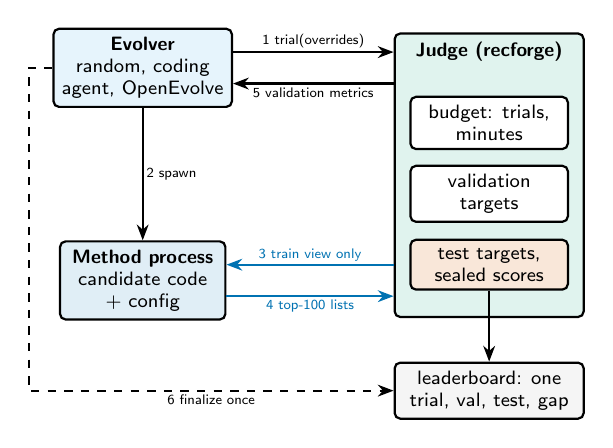
\begin{tikzpicture}[
  font=\sffamily\scriptsize,
  box/.style={draw, rounded corners=2pt, thick, align=center, inner sep=3pt},
  arr/.style={-{Stealth[length=2mm]}, thick},
  lab/.style={font=\sffamily\tiny, align=center, fill=white, inner sep=1pt},
]
\node[box, fill=cMeta!15, minimum width=21mm, minimum height=9mm] (ev) at (0,0) {\textbf{Evolver}\\random, coding\\agent, OpenEvolve};
\node[box, fill=cL2!12, minimum width=21mm, minimum height=9mm] (m) at (0,-27mm) {\textbf{Method process}\\candidate code\\+ config};
\node[box, fill=cL1!12, minimum width=24mm, minimum height=36mm, anchor=north] (j) at (44mm,4.5mm) {};
\node[anchor=north, font=\sffamily\scriptsize\bfseries] at (j.north) {Judge (recforge)};
\node[box, fill=white, minimum width=20mm] (bud) at (44mm,-7mm) {budget: trials,\\minutes};
\node[box, fill=white, minimum width=20mm] (val) at (44mm,-16mm) {validation\\targets};
\node[box, fill=cBad!15, minimum width=20mm] (test) at (44mm,-25mm) {test targets,\\sealed scores};
\node[box, fill=gray!8, minimum width=24mm] (lb) at (44mm,-41mm) {leaderboard: one\\trial, val, test, gap};

\draw[arr] ($(ev.east)+(0,2mm)$) -- node[lab, above] {1 trial(overrides)} ($(ev.east -| j.west)+(0,2mm)$);
\draw[arr] ($(ev.east -| j.west)+(0,-2mm)$) -- node[lab, below] {5 validation metrics} ($(ev.east)+(0,-2mm)$);
\draw[arr] (ev.south) -- node[lab, right] {2 spawn} (m.north);
\draw[arr, cL2] ($(m.east -| j.west)+(0,2mm)$) -- node[lab, above] {3 train view only} ($(m.east)+(0,2mm)$);
\draw[arr, cL2] ($(m.east)+(0,-2mm)$) -- node[lab, below] {4 top-100 lists} ($(m.east -| j.west)+(0,-2mm)$);
\draw[arr, dashed] (ev.west) -- ++(-3mm,0) |- node[lab, pos=0.75, below] {6 finalize once} (lb.west);
\draw[arr] (test) -- (lb);
\end{tikzpicture}
\caption{An evolve session in recforge. The evolver requests trials (1); each trial runs the candidate in its own
process (2), which receives a training view without targets (3) and returns ranked lists (4). Only validation
metrics flow back (5); test scores are computed and sealed. One \texttt{finalize} publishes a single trial with its
validation score, test score, gap and budget (6). The seal holds at the API level; file-system isolation is
planned.}
\label{fig:protocol}
\end{figure}


\begin{itemize}
\item \emph{One protocol per version.} The current protocol is leave-one-out per user (last item test,
second-to-last validation) with full-catalogue ranking, the user's history removed, and HR and NDCG at 10 and 20
and MRR@100 (items ranked below 100 score zero). Leave-one-out ignores the global timeline and can leak future
information~\cite{ji2020leakage,hidasi2023flaws}; a global temporal split is the next protocol version. Results from
different versions are never put in one table, and every result is keyed by the source hash of the method, its
configuration and the code commit.
\item \emph{A sealed test at the API level.} Method code runs in its own process and receives only a training view;
asking for a validation or test target raises an error, and the method returns ranked lists that the parent process
scores. The seal holds only against code that uses the API: sealed scores and session state are ordinary files, so
an agent with file-system access could read test scores or alter the budget. A container mode that would close this
gap (R8) is planned, not implemented.
\item \emph{Budgeted evolve sessions.} A session has a trial and time budget. Each trial returns validation metrics
only; test metrics are computed and sealed. A single \texttt{finalize} reveals the test metrics of exactly one
trial, publishes it with the session's budget, and closes the session.
\item \emph{Evolvers on equal terms.} An equal-budget random search (the R5 null), a wrapper for an external coding
agent, and an OpenEvolve adapter drive sessions through the same interface, and each run reports the
validation-to-test gap of its finalized trial. They are tested on synthetic data only; the OpenEvolve adapter has
not been run end to end.
\item \emph{Baselines and data.} Popularity, ItemKNN~\cite{sarwar2001itemknn}, BPR~\cite{rendle2009bpr},
SASRec~\cite{kang2018sasrec}, HSTU~\cite{zhai2024hstu} and TIGER~\cite{rajput2023tiger}, with
MovieLens-1M~\cite{harper2015movielens}, Amazon 2014 Beauty, Sports and Toys~\cite{mcauley2015amazon}, MIND
news~\cite{wu2020mind}, and the OpenOneRec release~\cite{zhou2025openonerec}.
\end{itemize}
Not yet implemented: the container mode, recording of LLM tokens and cost, automatic aggregation of repeated
sessions, and the temporal split.

\pdfinfo{/Author (Shanglin Yang; Zhan Shi) /Keywords (recommender systems, LLM agents, AutoML, program evolution, evaluation, reproducibility)}
\end{document}
